%!TEX root = ../thesis.tex
%*******************************************************************************
%****************************** Third Chapter **********************************
%*******************************************************************************
\chapter{A search for the Graviton in the \hhbbtmth channel}
\label{Chapter_Graviton}

\graphicspath{{1_MainChapters/Chap7_GravLimit/figures}{1_MainChapters/Chap7_GravLimit/notMyFigures}}


\section{Introduction}
    \label{sec:grav_intro}
    The Graviton is a spin-2 particle that mediates the gravitational force. 
    In addition to the RS model, the Graviton is also predicted by 
    other models such as string theory.
    The search for gravity in LHC boils down to a search for an undiscovered BSM heavy spin-2 particle ($G$).
    This type of search is sensitive to a broad range of other BSM theory, such as the Supersymmetry (SUSY) model,
    Two-Higgs Doublet Model (2HDM), the Composite Higgs Models (CHM), etc., which predict the existence of  
    spin-0 heavy scalar particles ($X$) that couple with the SM Higgs boson. Fig~\ref{fig:grav} shows the 
    Feynman diagram of the gluon--gluon production of the $X$ and $G$. These production processes are
    predicted to have the largest cross-section at the LHC, should they exist. The predicted cross-section of the
    $pp\rightarrow G\rightarrow HH$ production at the LHC centre of mass energies of 13~TeV and 13.6~TeV as functions of 
    the $G$ mass are shown in Fig~\ref{fig:grav_pred_xs}.
    \begin{figure}[htbp]
        \centering
        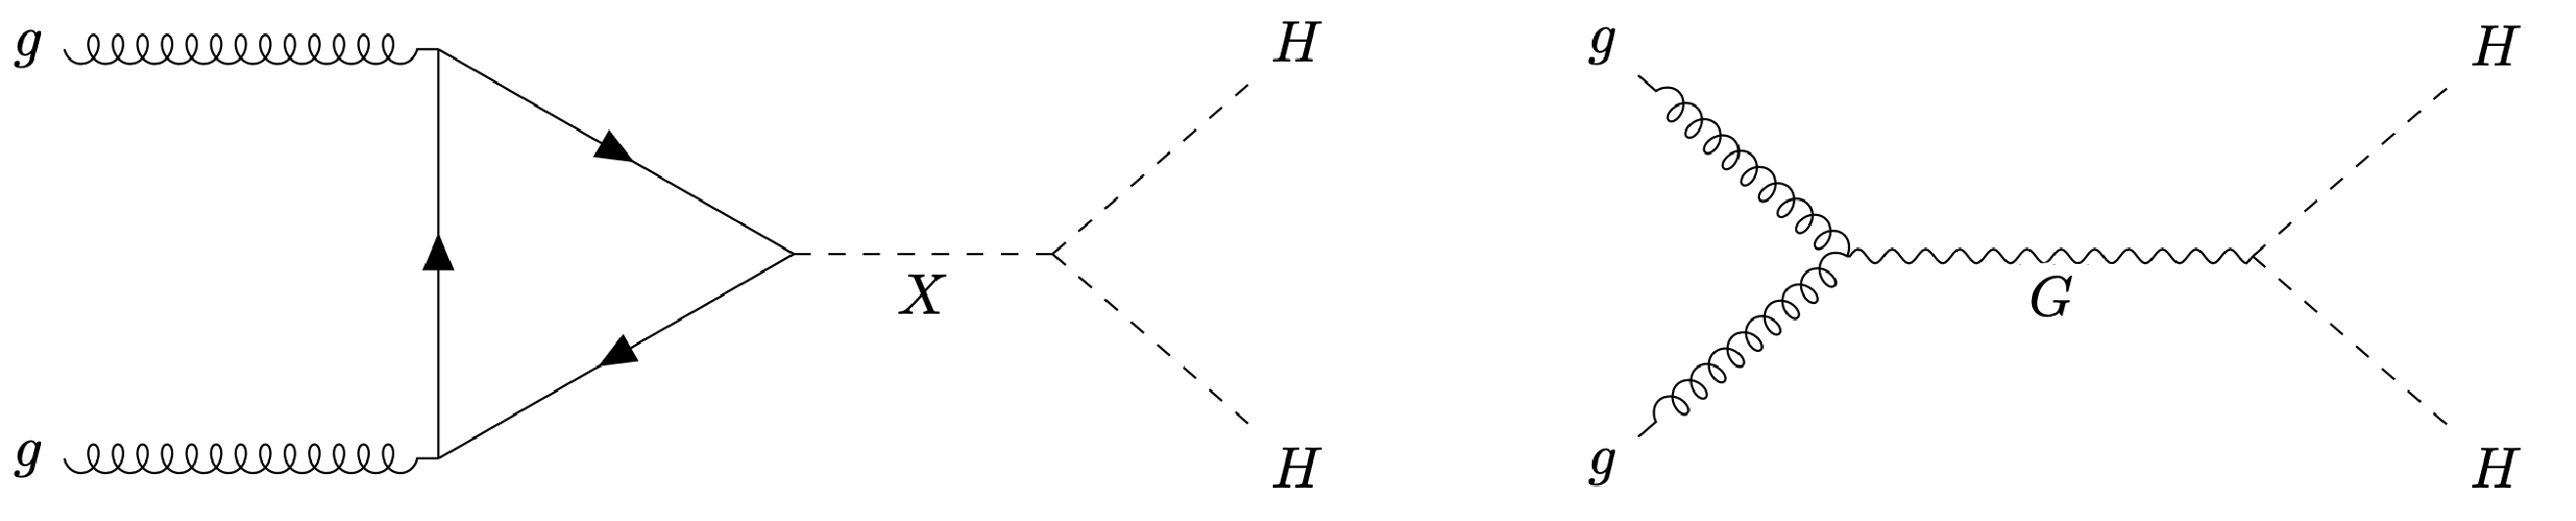
\includegraphics[width=1.0\textwidth]{GXHHFeynmanDiag.pdf}
        \caption{Feynman diagram of the gluon--gluon production of the $X$ and $G$.}
        \label{fig:grav}
    \end{figure}
    \begin{figure}[htbp]
        \centering
        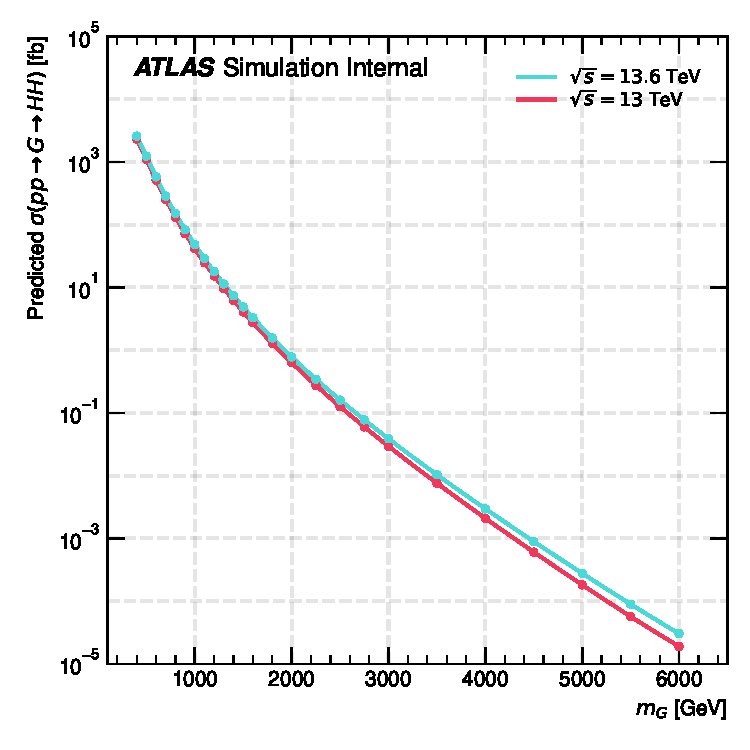
\includegraphics[width=0.5\textwidth]{GHH_prediction_xs.pdf}
        \caption{Predicted cross-section of the $pp\rightarrow G\rightarrow HH$ production at the LHC centre of mass energy of 13~TeV and 13.6~TeV.}
        \label{fig:grav_pred_xs}
    \end{figure}

    After the discovery of the Higgs boson, such searches have been performed extensively by ATLAS and CMS collaborations using Run-1 and Run-2 data, 
    but no evidence of new heavy particles has been found yet.
    In the $G/X\rightarrow HH$ channel, CMS published the combination \cite{CMS-B2G-23-002} of the 
    $\hhbbbb$~\cite{CMS-B2G-21-003}, 
    $\hhbbtt$~\cite{CMS-HIG-20-014}, 
    $\hhbbyy$~\cite{CMS-HIG-21-011}, 
    $\hhbbww$~\cite{CMS-HIG-21-005, CMS-B2G-20-007}, and 
    $\hhxxll$~\cite{CMS-HIG-21-002} searches using the full Run-2 data in 2024. 
    Prior to this, ATLAS published the Run-2 combination~\cite{HDBS-2023-17} of the resonant
    $\hhbbbb$~\cite{HDBS-2018-41}, 
    $\hhbbyy$~\cite{HDBS-2018-34}, and 
    $\hhbbtt$~\cite{HDBS-2018-40} searches in 2023, as well as a dedicated search for the highly boosted di-Higgs production in the $\hhbbthth$ channel 
    using the boosted $\tauhad\tauhad$ tagger~\cite{HDBS-2019-22}.
    \begin{table}[htbp]
    \caption{Summary of the expected and observed 95\% CL limits on the production cross-section of the di-higgs ($\sigma(G/X\rightarrow HH)$) set by ATLAS and CMS. 
        Limits are given in fb. The numbers inside and outside the brackets are the observed and the expected limits respectively.}
    \centering
    % \scriptsize
    \begin{tabular}{ll|rr|rr}
        \toprule
                                    &                   & \multicolumn{2}{c|}{CMS}                                   & \multicolumn{2}{c}{ATLAS}                                \\
        Mass                        & Channel           & $\sigma(X\rightarrow HH)$    & $\sigma(G\rightarrow HH)$   & $\sigma(X\rightarrow HH)$ & $\sigma(G\rightarrow HH)$    \\
        \midrule
        \multirow{4}{*}{1 TeV}      & Combined          & 5 (3)                            & 3 (2)                           & 6 (10)                          & N/A            \\
                                    & $\hhbbbb$         & 7 (5)                            & 3 (3)                           & 8 (7)                           & 8 (9)          \\
                                    & $\hhbbtt$         & 40 (22)                          & 1 (1)                           & 10 (30)                         & N/A            \\
                                    & $\hhbbyy$         & 10 (5)                           & 7 (3)                           & 50 (50)                         & N/A            \\
        \midrule                                                       
        \multirow{4}{*}{2 TeV}      & Combined          & 0.6 (0.5)                        & 0.4 (0.3)                       & 2 (3)                           & N/A            \\
                                    & $\hhbbbb$         & 0.7 (0.7)                        & 0.4 (0.4)                       & 2 (3)                           & 2 (3)          \\
                                    & $\hhbbtt$         & 140 (140)                        & N/A                             & 40 (50)                         & N/A            \\
                                    & $\hhbbyy$         & 2 (2)                            & 2 (1)                           & N/A                             & N/A            \\
        \midrule                                                       
        \multirow{4}{*}{3 TeV}      & Combined          & 0.5 (0.5)                        & 0.2 (0.2)                       & 1 (1)                           & N/A            \\
                                    & $\hhbbbb$         & 0.5 (0.5)                        & 0.2 (0.2)                       & 1 (1)                           & 1 (1)          \\
                                    & $\hhbbtt$         & 1400 (1400)                      & N/A                             & 50 (50)                         & N/A            \\
                                    & $\hhbbyy$         & 1 (1)                            & 1.0 (0.8)                       &  N/A                            & N/A            \\
        \midrule                                                       
        \multirow{4}{*}{4 TeV}      & Combined          & 0.3 (0.3)                        & N/A                             & 1 (3)                           & N/A            \\
                                    & $\hhbbbb$         & 0.4 (0.4)                        & N/A                             & 1 (3)                           & 1 (2)          \\
                                    & $\hhbbtt$         & N/A                              & N/A                             & N/A                             & N/A            \\
                                    & $\hhbbyy$         & 1 (1)                            & 0.8 (0.7)                       & N/A                             & N/A            \\
        \midrule                                                       
        \multirow{4}{*}{5 TeV}      & Combined          & 0.2 (0.3)                        & N/A                             & 1 (1)                           & N/A            \\
                                    & $\hhbbbb$         & 0.3 (0.3)                        & N/A                             & 1 (1)                           & 1 (1)          \\
                                    & $\hhbbtt$         & N/A                              & N/A                             & N/A                             & N/A            \\
                                    & $\hhbbyy$         & 1 (1)                            & N/A                             & N/A                             & N/A            \\
        \bottomrule
    \end{tabular}
    \label{tab:grav_cms}
\end{table}
    Table~\ref{tab:grav_cms} summarises the latest expected and observed 95\% CL limits on the production cross-section 
    of the di-Higgs ($\sigmaGHH$) set by ATLAS and CMS at 1 to 5 TeV mass points.  
    For both ATLAS and CMS, the $\hhbbbb$ channel is the most sensitive channel for the heavy resonance search in $G/X\rightarrow HH$ channels. This channel 
    has the highest branching ratio, and both collaborations have the most mature reconstruction techniques tagging highly boosted $b\bar{b}$ system~\cite{PERF-2017-04, CMS-DP-2020-002}.
    CMS has been taking the lead in the search in the $\hhbbbb$ and $\hhbbyy$ channel. On the other hand, ATLAS currently leads the search in the $\hhbbtt$ channel, 
    thanks to the boosted $\tauhad\tauhad$ tagger. 
    Compared to the predicted cross-sections, the upper limits set by 
    ATLAS and CMS collaborations have strongly excluded the existence of the Graviton 
    in the mass lower than 2 TeV. However, above 2 TeV, the limits set by the 
    both collaborations are still far higher than the predictions.

    We choose the muon-removal $\tauhad$ reconstruction ($\tauhadmurm$) as the boosted $\tmth$ tagger~\cite{Dong:2890038, Dong:2899443}. 
    The aim of such alternative reconstruction is to improve the $\tauhad$ reconstruction and identification efficiency in the boosted \tmth channel, as discussed in Chapter 5.
    In the meantime, the ATLAS boosted $b\bar{b}$ tagger incorporated graph neural networks (GNN)~\cite{ATL-PHYS-PUB-2023-021} 
    to significantly improve the boosted $b\bar{b}$ tagging (GN2x).
    In this chapter, we will present the search for the Graviton 
    in the \hhbbtmth channel with the 140~\ifb ATLAS Run-2 data. Using the $\tauhadmurm$ tagger and the newly developed GN2x boosted $b\bar{b}$ tagger~\cite{ATL-PHYS-PUB-2023-021},
    this analysis achieves the best sensitivity in the $\hhbbtt$ channel to date. The expected
    95\% CL limits on $\sigmaGHH$ for masses in the range 2-5 TeV are ten-times lower than the previous ATLAS search in the $\hhbbtt$ channel, more than 100 times lower than the
    expected limits set by the CMS collaboration in the same channel. 

    Section~\ref{sec:data_mc} describes the data and MC samples used in the analysis.
    Section~\ref{sec:grav:sel} describes the signal-region event-selection
    Section~\ref{sec:grav:sys} describes the systematic uncertainties considered in this analysis.
    Section~\ref{sec:grav:interp} describes the statistical analysis and limit setting.
    Section~\ref{sec:grav:conc} presents the results of the analysis and discusses the future prospects.


\section{Data and MC} \label{sec:data_mc}
    Full ATLAS Run-2 data was used in this analysis. The data collected at $\sqrt{s} = 13~\TeV$ corresponds to an integrated luminosity of $140~\ifb$. 
    For this analysis, the prediction for the SM contributions are from the same MC samples as those used for the $\tauhadmurm$ benchmark analysis detailed 
    in Chapter~5, with the exception of the addition of the SM Higgs and di-Higgs samples. 

    %boiler plate text from pmg
    %! ggF Higgs
    Higgs boson production via gluon--gluon fusion (ggF) was simulated at next-to-next-to-leading-order (NNLO) accuracy in 
    QCD using \POWHEGBOX[v2]~\cite{Hamilton:2013fea,Hamilton:2015nsa,Alioli:2010xd,Nason:2004rx,Frixione:2007vw}. 
    The simulation achieved NNLO accuracy for arbitrary inclusive $gg\to H$ observables by re-weighting the Higgs boson 
    rapidity spectrum in \textsc{Hj}-\MINLO~\cite{Hamilton:2012np,Campbell:2012am,Hamilton:2012rf} to that of HNNLO~\cite{Catani:2007vq}.
    %The transverse momentum spectrum of the Higgs boson obtained with this sample was found to be compatible with the fixed-order HNNLO calculation and the Hres2.3 calculation~\cite{Bozzi:2005wk,deFlorian:2011xf} performing resummation at next-to-next-to- leading-logarithm accuracy matched to a NNLO fixed-order calculation (NNLL+NNLO).
    The \PDFforLHC[15nnlo] PDF set~\cite{Butterworth:2015oua} and the \AZNLO tune~\cite{STDM-2012-23} 
    of \PYTHIA[8]~\cite{Sjostrand:2014zea} were used.
    The gluon--gluon fusion prediction from the Monte Carlo samples was normalised to the 
    next-to-next-to-next-to-leading-order cross-section in QCD plus electroweak corrections 
    at NLO~\cite{deFlorian:2016spz,Anastasiou:2016cez,Anastasiou:2015ema,Dulat:2018rbf,Harlander:2009mq,Harlander:2009bw,Harlander:2009my,Pak:2009dg,Actis:2008ug,Actis:2008ts,Bonetti:2018ukf,Bonetti:2018ukf}. 
    The normalisation of all Higgs boson
    samples accounts for the decay branching ratio calculated with HDECAY~\cite{Djouadi:1997yw,Spira:1997dg,Djouadi:2006bz}
    and \PROPHECY~\cite{Bredenstein:2006ha,Bredenstein:2006rh,Bredenstein:2006nk}.

    %! VBF Higgs
    Higgs boson production via vector-boson fusion was simulated with
    \POWHEGBOX[v2]~\cite{Nason:2009ai,Alioli:2010xd,Nason:2004rx,Frixione:2007vw} 
    and interfaced with \PYTHIA[8]~\cite{Sjostrand:2014zea} for parton shower and non-perturbative effects,
    with parameters set according to the \AZNLO tune~\cite{STDM-2012-23}.
    The \POWHEG prediction is accurate to next-to-leading order (NLO) and uses
    the \PDFforLHC[15nlo] PDF set~\cite{Butterworth:2015oua}. 
    It was tuned to match calculations with effects due to finite heavy-quark masses 
    and soft-gluon resummation up to NNLL.
    The Monte Carlo prediction was normalised to an approximate-NNLO QCD cross-section 
    with NLO electroweak corrections~\cite{Ciccolini:2007jr,Ciccolini:2007ec,Bolzoni:2010xr}. 
    The normalisation of all Higgs boson samples accounts for the decay branching ratio calculated 
    with \textsc{HDECAY}~\cite{Djouadi:1997yw,Spira:1997dg,Djouadi:2006bz} 
    and \PROPHECY~\cite{Bredenstein:2006ha,Bredenstein:2006rh,Bredenstein:2006nk}.

    %! VH
    Higgs boson production in association with a vector boson was simulated using
    \POWHEGBOX[v2]~\cite{Nason:2009ai,Alioli:2010xd,Nason:2004rx,Frixione:2007vw} and interfaced with \PYTHIA[8]~\cite{Sjostrand:2014zea} for
    parton shower and non-perturbative effects. The \POWHEG prediction is accurate to next-to-leading order for $VH$ boson plus one-jet production. 
    The loop-induced $gg\to ZH$ process was generated separately at leading order. The \PDFforLHC[15nlo] PDF
    set~\cite{Butterworth:2015oua} and the \AZNLO tune~\cite{STDM-2012-23} of \PYTHIA[8]~\cite{Sjostrand:2014zea} were used. The Monte Carlo
    prediction was normalised to cross-sections calculated at NNLO in QCD with NLO electroweak corrections for $q\bar{q}/qg \to VH$ and at NLO
    and next-to-leading-logarithm accuracy in QCD for $gg \to
    ZH$~\cite{Ciccolini:2003jy,Brein:2003wg,Brein:2011vx,Altenkamp:2012sx,Denner:2014cla,Brein:2012ne,Harlander:2014wda}. The
    normalisation of all Higgs boson samples accounts for the decay branching ratio calculated with 
    HDECAY~\cite{Djouadi:1997yw,Spira:1997dg,Djouadi:2006bz} and \PROPHECY~\cite{Bredenstein:2006ha,Bredenstein:2006rh,Bredenstein:2006nk}.

    %! dihiggs
    The ggF production of the SM Higgs boson pairs, with one Higgs boson decaying into $b\bar{b}$ 
    and the other one to $\tau^+\tau^-$ is generated with the Powheg Box v2 generator at 
    NLO with finite top-quark mass, and using the \PDFforLHC[15nlo]
    PDFset. Parton shower and hadronisation are simulated using \PYTHIA[8.244]~\cite{Sjostrand:2014zea}
    with the A14 tune and the \NNPDF[2.3lo]~\cite{Ball:2012cx} PDF set. 

    %! signals
    The $\GHHbbtt$ signal samples are generated with the same setup as the $\GHHFourtau$ samples in the $\tauhadmurm$ development, detailed in Chapter 5.
    To enhance the statistics, the Higgs bosons in the signal $\GHHbbtt$ samples are forced to decay to a pair of $b$-quarks or a pair of $\tau$-leptons, in equal branching fractions.
    To calculate the effective cross-sections for the $G\rightarrow HH$ production, a scale factor of 
    $$\frac{\mathrm{BR}_\mathrm{SM}(\hhbbtt)}{\mathrm{BR}_\mathrm{Gen}(\hhbbtt)} = \frac{0.073}{0.5} = 0.146$$ 
    was applied to the generator reported cross-sections,
    where $\mathrm{BR}_\mathrm{SM}(\hhbbtt) = 0.073$ is the SM branching ratio of the $\hhbbtt$ decay, 
    and $\mathrm{BR}_\mathrm{Gen}(\hhbbtt) = 0.5$ is the generator-enhanced branching ratio for the same process.

\section{Event-selection}
    \label{sec:grav:sel}
    \begin{table}[htbp]
    \caption{Summary of signal region event-selection criteria. SR events pass at least one trigger listed below. 
    A control region is defined in which events fail any one or more of the cuts marked with \textbf{*}, while passing every other selection.
    For better CR statistics, the lower bound of $\mttcol$ and $\mbb$ is relaxed to 60 GeV for CR.
    ``fatjet'' refers to the large-radius jet clustered with the anti-$k_t$ algorithm with $R=1.0$.
    }
    \label{tab:evt_sel}
    \centering
    % \scriptsize
    \begin{tabular}{lr}
    \toprule
    Object & \begin{tabular}{rr} Selection & \end{tabular} \\
    \midrule
    Triggers                & \begin{tabular}{rr} 
                                lowest un-prescaled single muon triggers &  \\ 
                                lowest un-prescaled $\met$ triggers &  \\
                            \end{tabular} \\
    \midrule
    $\tauhadmurm$           & \begin{tabular}{rr} 
                                $0 < |\eta| < 1.37$ or $1.52 < |\eta| < 2.5$ &  \\ 
                                "VeryLoose" RNN jet WP &  \\
                                $\pT > 20~\GeV$ &  \\
                            \end{tabular}   \\
    \midrule
    Removed $\mu$           & \begin{tabular}{rr} 
                                Found inside the \tauhadmurm &  \\ 
                                $\pt > 10~\GeV$  &  \\ 
                                "Medium" ID WP  &  
                            \end{tabular} \\
    \midrule
    $\mathrm{bb}$ system    & \begin{tabular}{rr} 
                                fatjet GN2x score > -5.0 &  \\
                                fatjet passes "QCD1.55\%" WP & \textbf{*} \\ 
                                $90 < \mbb < 160~\GeV$ & \\ 
                                $\ptbb > 250~\GeV$ & \\ 
                                $\dRjfj < 0.03$ & \textbf{*} 
                            \end{tabular} \\
    \midrule
    $\tmth$ system          & \begin{tabular}{rr} 
                                Opposite sign $\mu$ and $\tauhadmurm$ & \textbf{*} \\ 
                                $\mttvis > 5~\GeV$ &  \\ 
                                -0.1 < $\dPhiMuMet$ < 0.4 &  \\ 
                                $\mttcol > 90~\GeV$ &  \\ 
                                $\pttt > 250~\GeV$ &  
                            \end{tabular}  \\
    \midrule
    Event level cut         & \begin{tabular}{rr} 
                                $\absdPhibbtt > \pi/2$ &  \\
                                % $\mbbttcol > 1200~\GeV$ & \\
                            \end{tabular}  \\
    \bottomrule
    \end{tabular}
\end{table}

    
\begin{table}[htbp]
    \caption{Event yields in the SR and CR regions. The uncertainties are statistical only. 
    The signal yields are shown with fixed cross-sections $\sigma(pp\rightarrow G\rightarrow HH) = 1$ fb.}
    \label{tab:n_evt}
    \centering
    % \scriptsize
    \begin{tabular}{lrr}
        \toprule
                                                            & SR                   & CR                 \\
        \midrule
        Data                                                & $1 \pm 1$             & $219   \pm 15$      \\ 
        SM MC total                                         & $0.71  \pm 0.09$      & $205   \pm 2$     \\
        \midrule
        jets + $Z\rightarrow\tau\tau$                       & $0.19  \pm 0.05$      & $114   \pm 1$       \\
        diBoson                                             & $0.11  \pm 0.02$      & $16.1  \pm 0.4$     \\  
        Top                                                 & $0.12  \pm 0.03$      & $46    \pm 2$       \\
        Higgs                                               & $0.12  \pm 0.07$      & $11    \pm 1$       \\
        Others                                              & $0.168 \pm 0.005$     & $18    \pm 2$       \\
        \midrule
        $G(2~\TeV)\rightarrow HH$                           & $0.515  \pm 0.002$    & $0.178  \pm 0.001$  \\
        $G(3~\TeV)\rightarrow HH$                           & $0.712  \pm 0.002$    & $0.173  \pm 0.001$  \\
        $G(4~\TeV)\rightarrow HH$                           & $0.748  \pm 0.002$    & $0.196  \pm 0.001$  \\
        $G(5~\TeV)\rightarrow HH$                           & $0.728  \pm 0.002$    & $0.218  \pm 0.001$  \\
        \bottomrule
    \end{tabular}
\end{table}
    % 
\begin{table}[htbp]
    \caption{Summary of triggers used in the analysis. The lowest un-prescaled single muon triggers and $\met$ triggers are used. Events are required to pass at least one trigger.}
    \label{tab:triggers}
    \centering
    % \scriptsize
    \begin{tabular}{lr}
        \toprule
        Year & \begin{tabular}{r} Trigger\end{tabular} \\
        \midrule
        2015 & \begin{tabular}{r} 
                    \texttt{HLT\_xe70\_mht}\\ 
                    \texttt{HLT\_mu20\_iloose\_L1MU15}\\
                    \texttt{HLT\_mu50}\\
                \end{tabular} \\
        \midrule
        2016 & \begin{tabular}{r} 
                    \texttt{HLT\_xe110\_mht\_L1XE50}\\
                    \texttt{HLT\_mu26\_ivarmedium}\\
                    \texttt{HLT\_mu50}\\
                \end{tabular} \\
        \midrule
        2017 & \begin{tabular}{r} 
                    \texttt{HLT\_xe110\_pufit\_L1XE55}\\
                    \texttt{HLT\_mu26\_ivarmedium}\\
                    \texttt{HLT\_mu50}\\
                \end{tabular} \\
        \midrule
        2018 & \begin{tabular}{r} 
                    \texttt{HLT\_xe110\_pufit\_xe70\_L1XE50} \\ 
                    \texttt{HLT\_mu26\_ivarmedium}\\
                    \texttt{HLT\_mu50}\\
                \end{tabular} \\
        \bottomrule
    \end{tabular}
\end{table}


    The event-selection criteria are summarised in Table~\ref{tab:evt_sel}. 
    Recorded events are required to satisfy the same triggers as the $\tauhadmurm$ benchmark analysis detailed in Chapter~5.
    The signal-region events are required to have at least one $\tauhadmurm$ candidate with 
    $\pt > 20~\GeV$ and pseudorapidity satisfying $0 < |\eta| < 1.37$ or $1.52 < |\eta| < 2.5$. 
    A ``VeryLoose'' RNN jet WP is applied to the $\tauhadmurm$ candidate. 
    The removed muon is required to have $\pt > 10~\GeV$ and to pass the ``Medium'' ID WP.
    The fatjet is required to have a GN2x score greater than $-5.0$ and to pass the ``QCD1.55\%'' GN2x WP~\cite{ATL-PHYS-PUB-2023-021}. 
    The invariant mass of the $b\bar{b}$ system, $\mbb$, is required to be between 90 and 160~GeV, 
    and the \pt of the $b\bar{b}$ system, $\ptbb$, is required to be greater than 250~GeV. 
    The $\Delta{R}$ separation between the fatjet and the closest standard-radius jet, $\dRjfj$, is required to be less than 0.03.
    The $\tmth$ system is required to consist of an oppositely charged muon and $\tauhadmurm$ candidate, 
    and the visible mass of the $\tmth$ system, $\mttvis$, is required to be greater than 5~GeV. 
    The signed angular separation in the transverse plane between the muon and the $\MET$, $\dPhiMuMet$, 
    is required to be between $-0.1$ and $0.4$. 
    The invariant mass of the $\tmth$ system, $\mttcol$, is required to be greater than 90~GeV, 
    and the \pt of the $\tmth$ system, $\pttt$, is required to be greater than 250~GeV.
    At the event level, the absolute angular separation in $\phi$ between the $b\bar{b}$ system and the $\tmth$ system, 
    $\absdPhibbtt$, is required to be greater than $\pi/2$. 
    For the CR, the lower bounds of $\mttcol$ and $\mbb$ are relaxed to 60~GeV to increase the statistics. 
    Events that fail any one or more of the GN2x requirements, 
    the opposite-sign muon and $\tauhadmurm$ requirement, 
    or the $\dRjfj$ requirement, while passing all other selections, 
    are defined as belonging to the CR. 

    \subsection{$\mbb$ and $\mttcol$ cuts optimisation}
        The $\mbb$ and $\mttcol$ distributions are two powerful discriminants for the $G \rightarrow HH$ signal. 
        To maximise the sensitivity of the analysis, the cut values on the $\mbb$ and $\mttcol$ distributions are determined at pre-selection level.
        All other event-selection criteria are applied except for the $\mbb$ and $\mttcol$ cuts during the optimisation. 
        The signal and background efficiencies and the significance ($Z$) for different cut values on the 
        $\mbb$ and $\mttcol$ distributions are shown in Figure~\ref{fig:G3000_opt}.
        Due to the low number of expected events, the p-value is calculated using an interpolated Poisson 
        cumulative distribution function (CDF). 
        Then, $Z$ is derived from the p-value using $Z = \Phi^{-1}(1 - p)$, where $\Phi$ is the CDF of the standard normal distribution. 
        The optimal cut values are chosen to maintain high signal efficiencies and high significance. 
        The values of the optimal cuts are chosen to be looser than the values that maximise $Z$, 
        as $\mbb$ and $\mttcol$ are not the most powerful discriminants for the $G \rightarrow HH$ signal. 
        The $\mbbttcol$ distribution provides better separation between the signal and background, especially for the high-mass signals.

        % \begin{figure}[htbp]
        %     \centering
        %     \subfloat[]{
        %         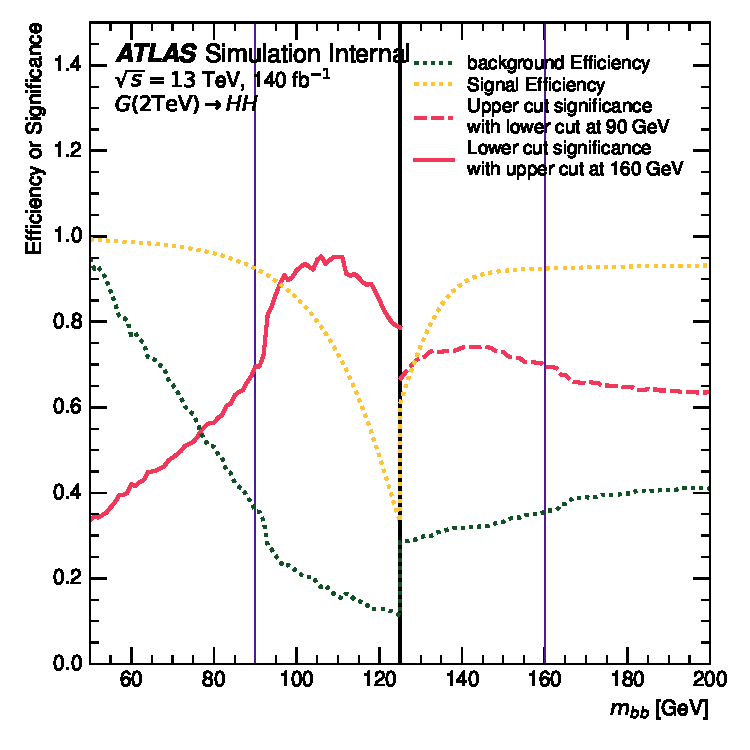
\includegraphics[width=0.50\textwidth]{cutOpt/signal_G2000_M_bb.pdf}
        %         \label{fig:G2000_mbb}
        %     }
        %     %\hfill
        %     \subfloat[]{
        %         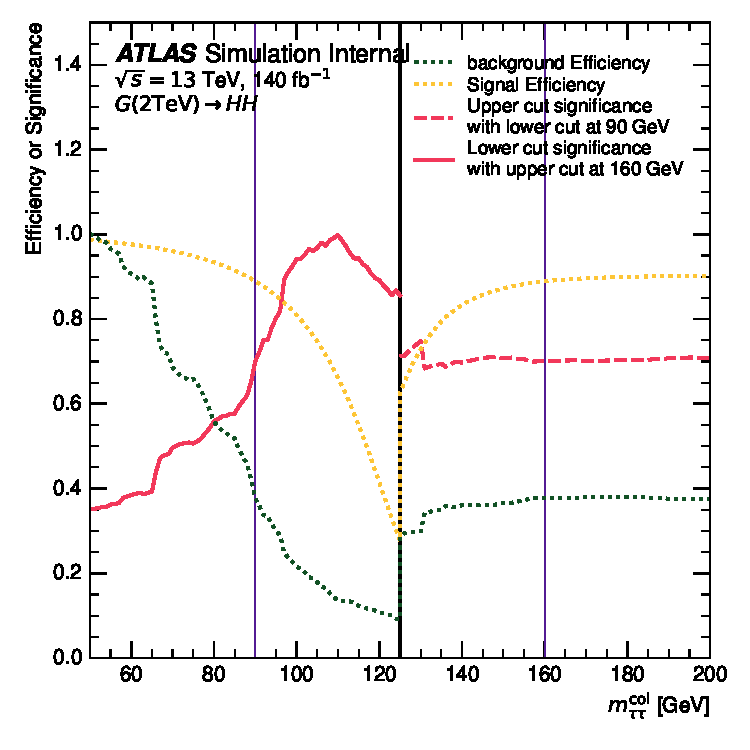
\includegraphics[width=0.50\textwidth]{cutOpt/signal_G2000_M_tt.pdf}
        %         \label{fig:G2000_mtt}
        %     }
        %     \caption{
        %         The $G~\text{2 TeV}$ signal efficiency, background efficiency, and the significance for different cut values on the 
        %         $\mbb$ \protect\subref{fig:G2000_mbb}, and $\mttcol$ \protect\subref{fig:G2000_mtt} distributions.
        %     }
        %     \label{fig:G2000_opt}
        % \end{figure}
        \begin{figure}[htbp]
            \centering
            \subfloat[]{
                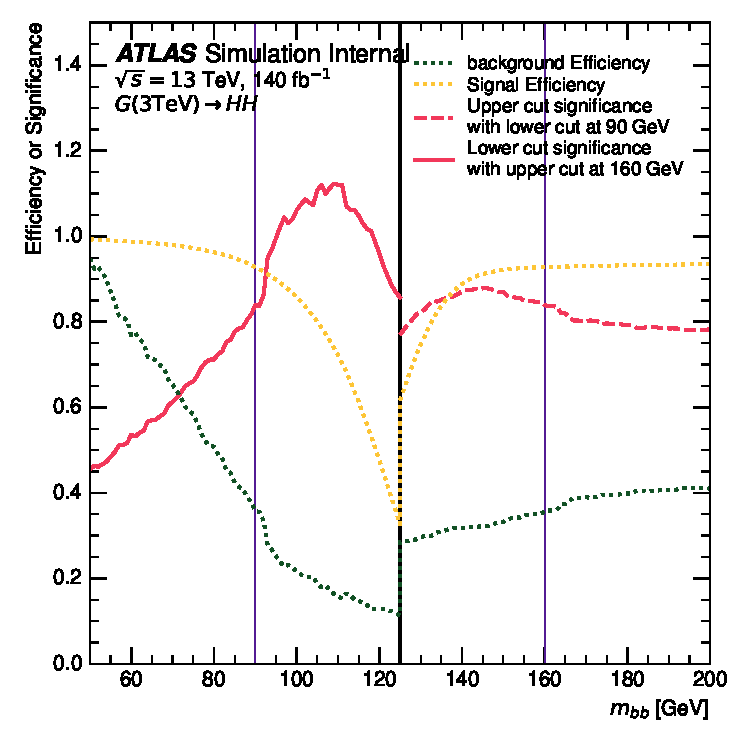
\includegraphics[width=0.50\textwidth]{cutOpt/signal_G3000_M_bb.pdf}
                \label{fig:G3000_mbb}
            }
            %\hfill
            \subfloat[]{
                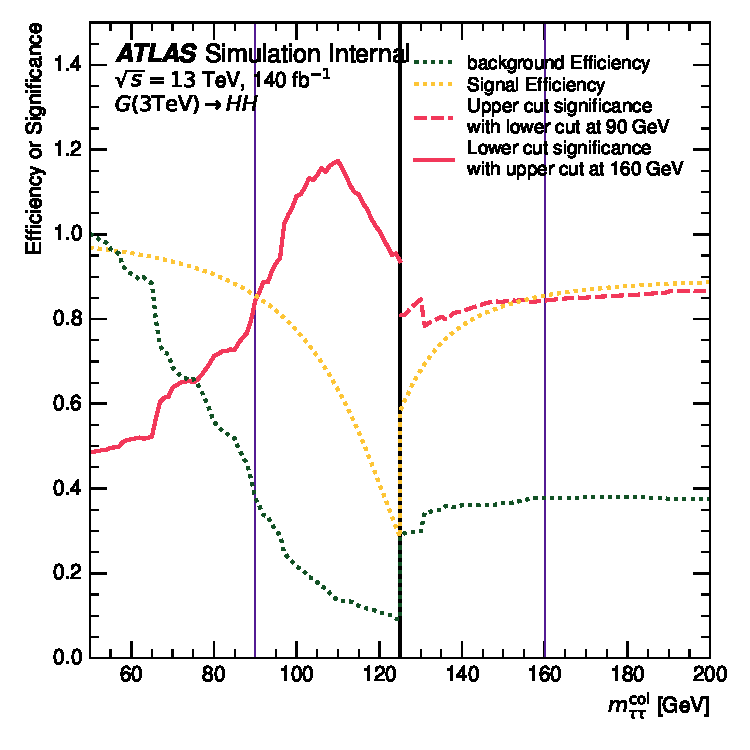
\includegraphics[width=0.50\textwidth]{cutOpt/signal_G3000_M_tt.pdf}
                \label{fig:G3000_mtt}
            }
            \caption{
                The $G~\text{3 TeV}$ signal efficiency, background efficiency, and the significance for different cut values on the 
                $\mbb$ (\protect\subref{fig:G3000_mbb}), and $\mttcol$ (\protect\subref{fig:G3000_mtt}) distributions.
            }
            \label{fig:G3000_opt}
        \end{figure}
        % \begin{figure}[htbp]
        %     \centering
        %     \subfloat[]{
        %         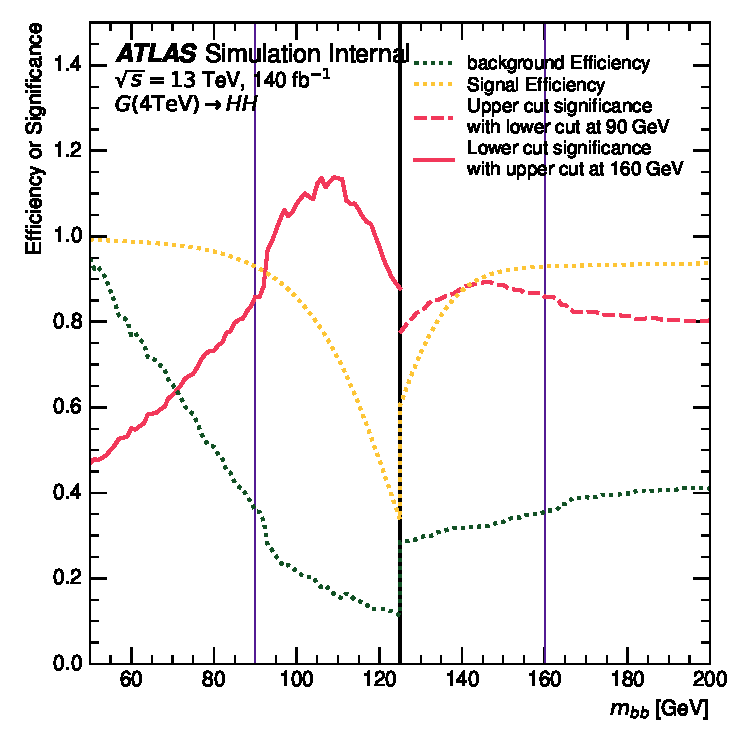
\includegraphics[width=0.50\textwidth]{cutOpt/signal_G4000_M_bb.pdf}
        %         \label{fig:G4000_mbb}
        %     }
        %     %\hfill
        %     \subfloat[]{
        %         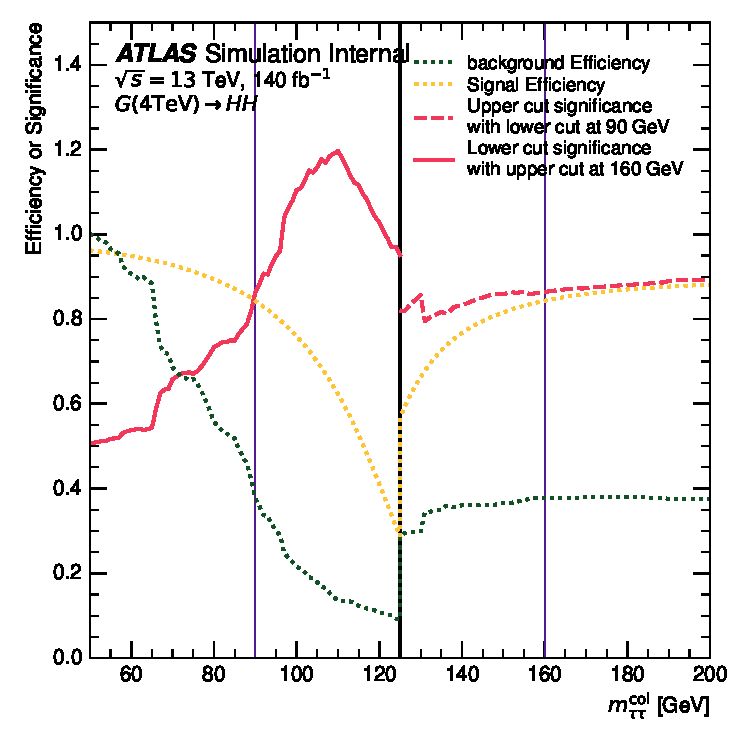
\includegraphics[width=0.50\textwidth]{cutOpt/signal_G4000_M_tt.pdf}
        %         \label{fig:G4000_mtt}
        %     }
        %     \caption{
        %         The $G~\text{4 TeV}$ signal efficiency, background efficiency, and the significance for different cut values on the 
        %         $\mbb$ \protect\subref{fig:G4000_mbb}, and $\mttcol$ \protect\subref{fig:G4000_mtt} distributions.
        %     }
        %     \label{fig:G4000_opt}
        % \end{figure}
        % \begin{figure}[htbp]
        %     \centering
        %     \subfloat[]{
        %         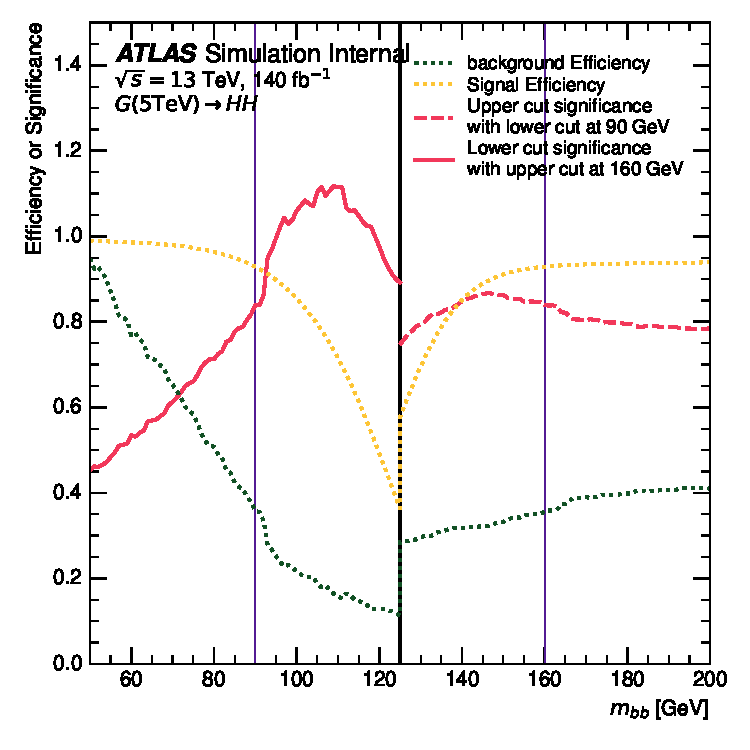
\includegraphics[width=0.50\textwidth]{cutOpt/signal_G5000_M_bb.pdf}
        %         \label{fig:G5000_mbb}
        %     }
        %     %\hfill
        %     \subfloat[]{
        %         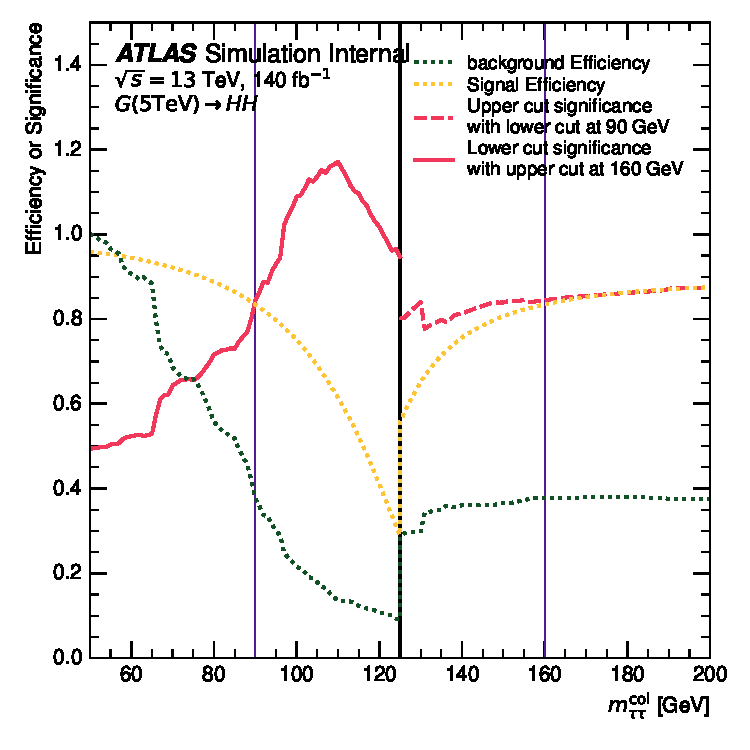
\includegraphics[width=0.50\textwidth]{cutOpt/signal_G5000_M_tt.pdf}
        %         \label{fig:G5000_mtt}
        %     }
        %     \caption{
        %         The $G~\text{5 TeV}$ signal efficiency, background efficiency, and the significance for different cut values on the 
        %         $\mbb$ \protect\subref{fig:G5000_mbb}, and $\mttcol$ \protect\subref{fig:G5000_mtt} distributions.
        %     }
        %     \label{fig:G5000_opt}
        % \end{figure}


\section{Results}
    \label{sec:grav:res}
    Figures~\ref{fig:absDphi_bbtt} to \ref{fig:tau_rnn} show the distributions of various variables in the SR and CR. 
    ``$Z\rightarrow\tau\tau$+jets'' refers to the contributions of the $Z\rightarrow\tau\tau$+jets processes.
    ``Top'' refers to the contributions of the SM top quark processes, including $t\bar{t}$ and single top.
    ``VV/VH/HH'' refers to the contributions of the SM diboson, $VH$, and $HH$ processes.
    ``Higgs'' refers to the contributions of the SM Higgs boson processes, including ggF and VBF productions.
    ``Other'' refers to the contributions of the remaining SM processes, including $W$+jets and $Z\rightarrow ll$+jets.
    The signal processes shown in these plots are normalised to the expected 95\% confidence level (CL) limits of the $\sigmaGHH$. 
    For variables used in the event-selection, these plots display the distributions after all other 
    event-selections have been applied, except for the variable itself. 
    The event yields in the SR and CR regions are presented in Table~\ref{tab:n_evt}. 
    Good agreement between data and MC simulation is observed in the CR, 
    indicating that the MC prediction is reliable in this region. 
    It also suggests negligible QCD background contamination in both the CR and SR.
    Figure~\ref{fig:absDphi_bbtt} shows the distribution of \absdPhibbtt between the two $b$-jets and the two $\tau$-leptons. 
    Figure~\ref{fig:dPhi_mu_met} displays the distribution of the $\dPhiMuMet$ variable. 
    The sign of $\dPhiMuMet$ is defined to be positive if the $\MET$ is on the same side as the $\tauhadmurm$ candidate, and negative otherwise. 
    Figure~\ref{fig:dR_jfj} illustrates the \dRjfj distributions. 
    This variable is utilised to reject events exhibiting significant 
    activity in the periphery of the fatjet, which often indicates the presence of gluon-induced heavy-flavour jets.
    Figure~\ref{fig:GN2bb} shows the distribution of the $\GNTwoXFj$ variable, which is the output of the GN2x tagger. 
    The WP chosen for this analysis is the ``QCD1.55\%'' WP, corresponding to a signal efficiency of 85\%. 
    Figures~\ref{fig:mbb} and \ref{fig:pTbb} present the distributions of \mbb\ and \ptbb\ of the two $b$-jets derived from the fatjet. 
    Figures~\ref{fig:mtt} and \ref{fig:pTtt} show the distributions of \mttcol\ and \pttt\ of the two $\tau$-leptons reconstructed with the collinear approximation~\cite{Dong:2890038, Dong:2899443}, incorporating the $\MET$. 
    The \ptbb\ and \pttt\ of Standard Model (SM) backgrounds fall sharply with increasing $\pt$, while the signal processes peak at $\frac{1}{2}m_G$.
    The signal \mbb\ and \mttcol\ distributions exhibit a clear peak at $m_H$.
    SM ``VV/VH/HH'' processes show broad distributions in the \mbb\ and \mttcol\ spectra from $m_Z$ to $m_H$. The contribution from top quark processes is clearly visible in the \mbb\ around 175~GeV. 
    A clear peak at $m_Z$ is observed in the \mttcol\ distribution from the $Z\rightarrow\tau\tau$+jets processes, indicating that the $Z$ + heavy flavour jets processes are well modelled in the high-\pt region.
    Other SM processes display falling distributions in the \mbb\ and \mttcol\ spectra.
    Figure~\ref{fig:mbbtt} shows the distribution of the $\mbbttcol$ variable, which is the invariant mass of the $b\bar{b}$ system and the two $\tau$-leptons. 
    This variable reconstructs the di-Higgs mass in the signal process. 
    Non-resonant SM processes exhibit falling distributions in the \mbbttcol\ spectra, 
    while the signal processes show a clear peak at $m_G$. 
    The lower tails of the \mbbttcol\ distributions from high-mass signals indicate poor detector resolution in the high-mass region. 
    Figure~\ref{fig:pTmu} presents the distribution of the $\pt$ of the muon found inside the $\tauhadmurm$ (\ptmuon). 
    Figure~\ref{fig:tau_rnn} displays the distribution of the TauID jet RNN score (\rnn) of the $\tauhadmurm$ candidate. 
    Figure~\ref{fig:qq} shows the distribution of the product of the $\tmth$ charges.

    \begin{figure}[htbp]
        \centering
        \subfloat[]{
            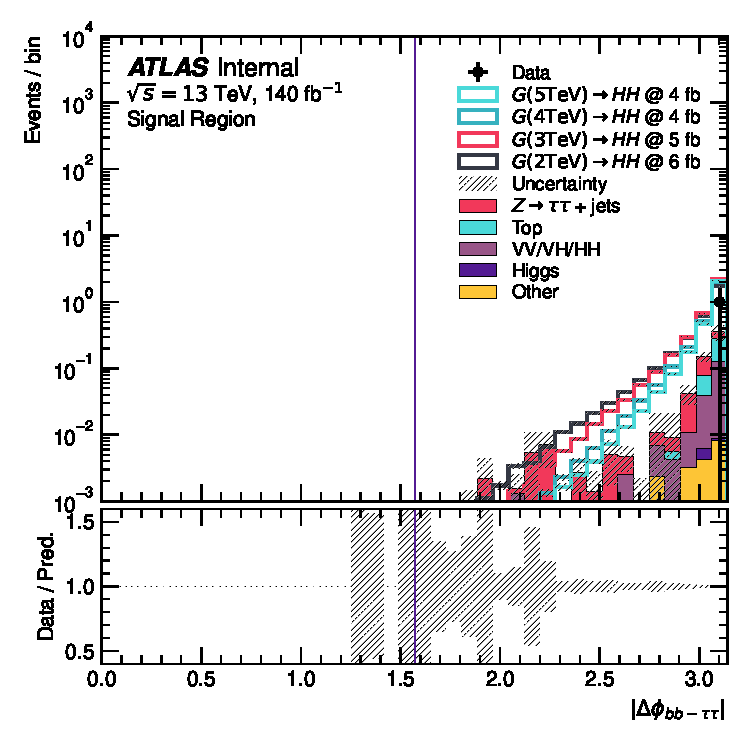
\includegraphics[width=0.50\textwidth]{kinematics_ub/abs_dPhi_bb_tt_SR.pdf}
            \label{fig:SR_absDphi_bbtt}
        }
        %\hfill
        \subfloat[]{
            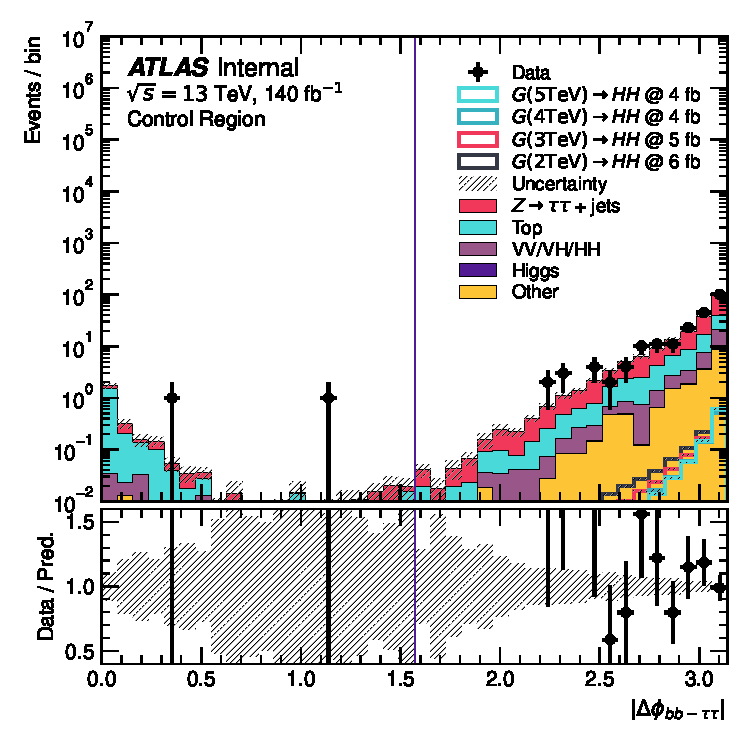
\includegraphics[width=0.50\textwidth]{kinematics_ub/abs_dPhi_bb_tt_CR.pdf}
            \label{fig:CR_absDphi_bbtt}
        }
        \caption{
            The distribution of the $\absdPhibbtt$ in the SR (\protect\subref{fig:SR_absDphi_bbtt}), and CR (\protect\subref{fig:CR_absDphi_bbtt}).
        }    
        \label{fig:absDphi_bbtt}
    \end{figure}

    \begin{figure}[htbp]
        \centering
        \subfloat[]{
            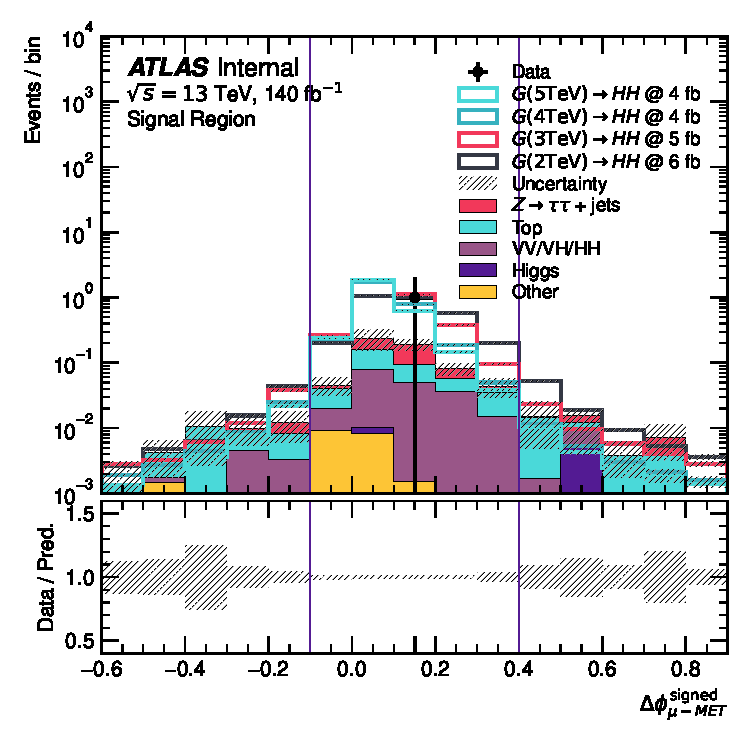
\includegraphics[width=0.50\textwidth]{kinematics_ub/dPhi_mu_met_SR.pdf}
            \label{fig:SR_dPhi_mu_met}
        }
        %\hfill
        \subfloat[]{
            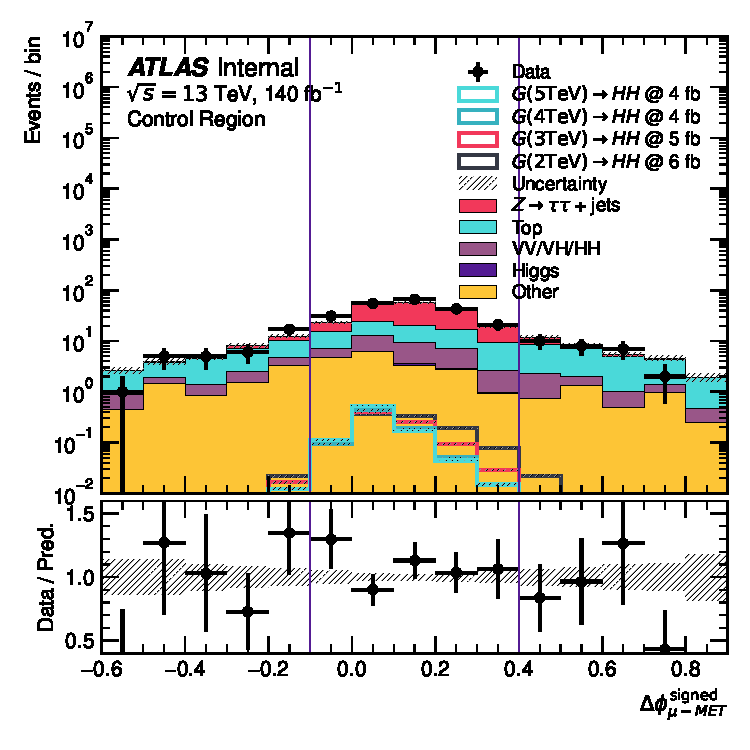
\includegraphics[width=0.50\textwidth]{kinematics_ub/dPhi_mu_met_CR.pdf}
            \label{fig:CR_dPhi_mu_met}
        }
        \caption{
            The distribution of the $\dPhiMuMet$ in the SR (\protect\subref{fig:SR_dPhi_mu_met}), and CR (\protect\subref{fig:CR_dPhi_mu_met}).
        }
        \label{fig:dPhi_mu_met}
    \end{figure}

    \begin{figure}[htbp]
        \centering
        \subfloat[]{
            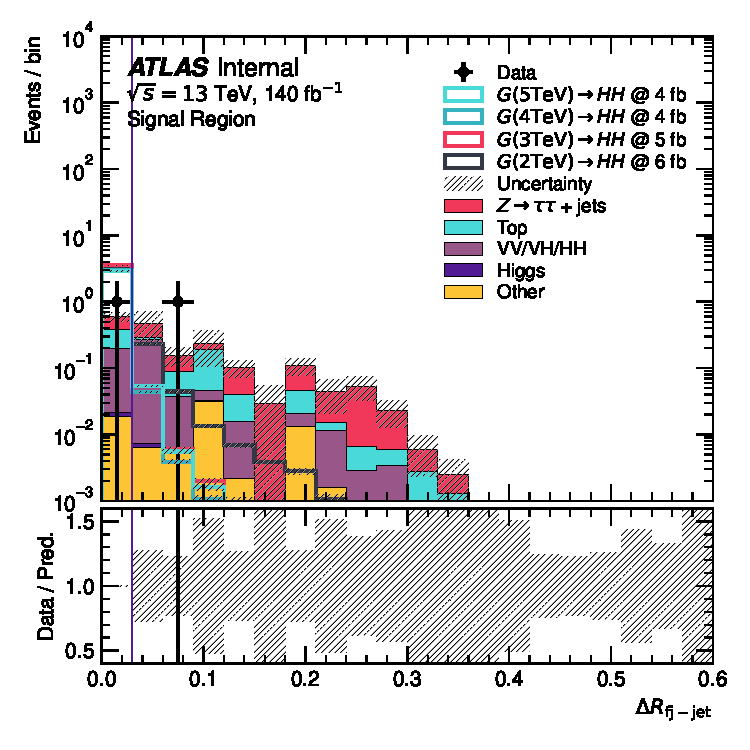
\includegraphics[width=0.50\textwidth]{kinematics_ub/dR_fj_jet_SR.pdf}
            \label{fig:SR_dR_jfj}
        }
        %\hfill
        \subfloat[]{
            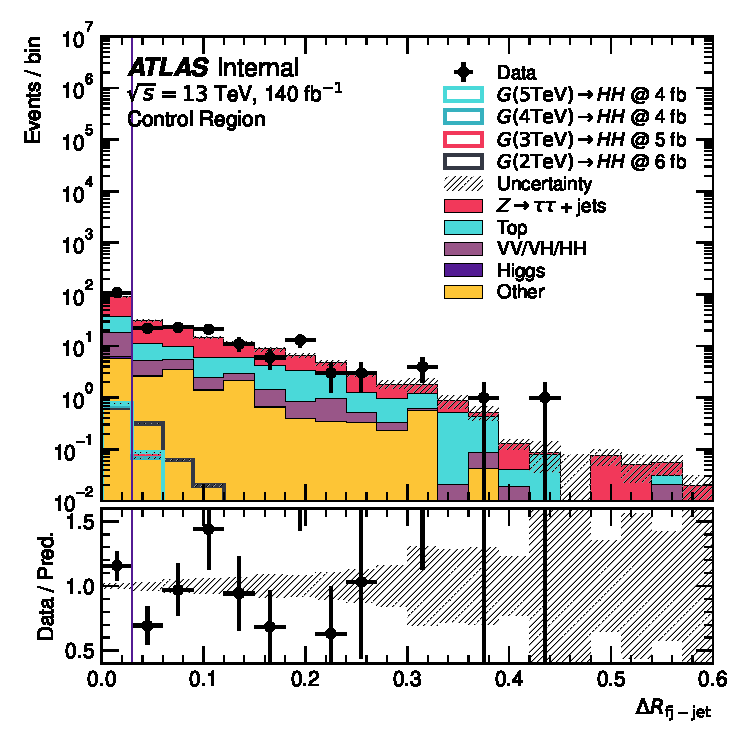
\includegraphics[width=0.50\textwidth]{kinematics_ub/dR_fj_jet_CR.pdf}
            \label{fig:CR_dR_jfj}
        }
        \caption{
            The distribution of the $\dRjfj$ in the SR (\protect\subref{fig:SR_dR_jfj}), and CR (\protect\subref{fig:CR_dR_jfj}).
        }
        \label{fig:dR_jfj}
    \end{figure}

    \begin{figure}[htbp]
        \centering
        \subfloat[]{
            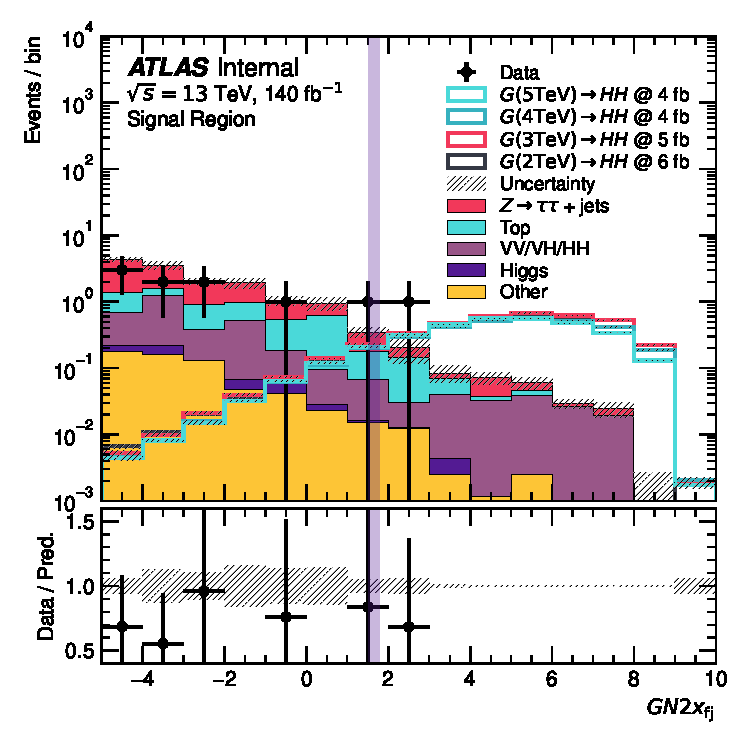
\includegraphics[width=0.50\textwidth]{kinematics_ub/fj_GN2x_SR.pdf}
            \label{fig:SR_GN2bb}
        }
        %\hfill
        \subfloat[]{
            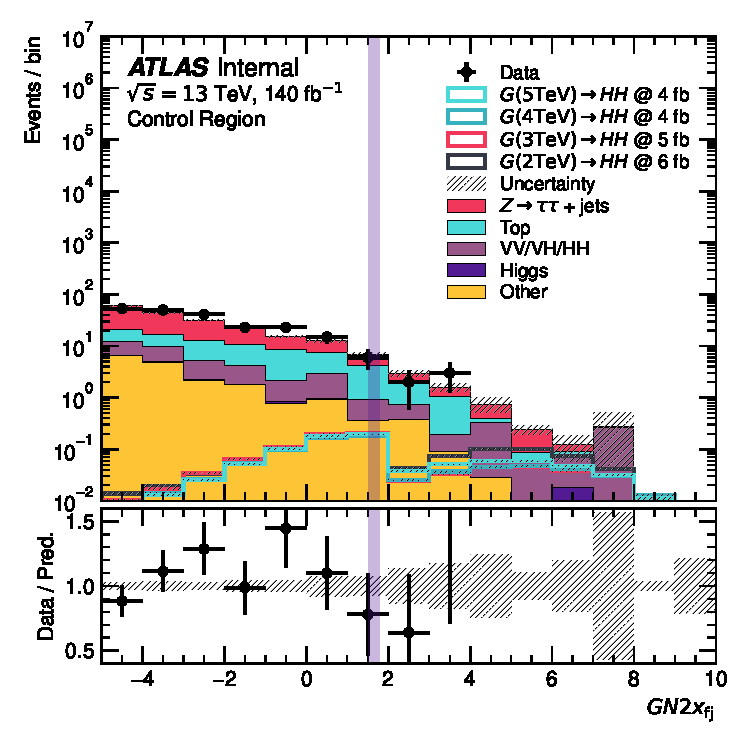
\includegraphics[width=0.50\textwidth]{kinematics_ub/fj_GN2x_CR.pdf}
            \label{fig:CR_GN2bb}
        }
        \caption{
            The distribution of the $\GNTwoXFj$ in the SR (\protect\subref{fig:SR_GN2bb}), and CR (\protect\subref{fig:CR_GN2bb}). 
            The translucent band indicates the cut value of ``QCD1.55\%'' GN2x WP, ranging from 1.6 to 1.7 in the region where the fatjet mass is between 90 and 160 GeV.
        }
        \label{fig:GN2bb}
    \end{figure}

    \begin{figure}[htbp]
        \centering
        \subfloat[]{
            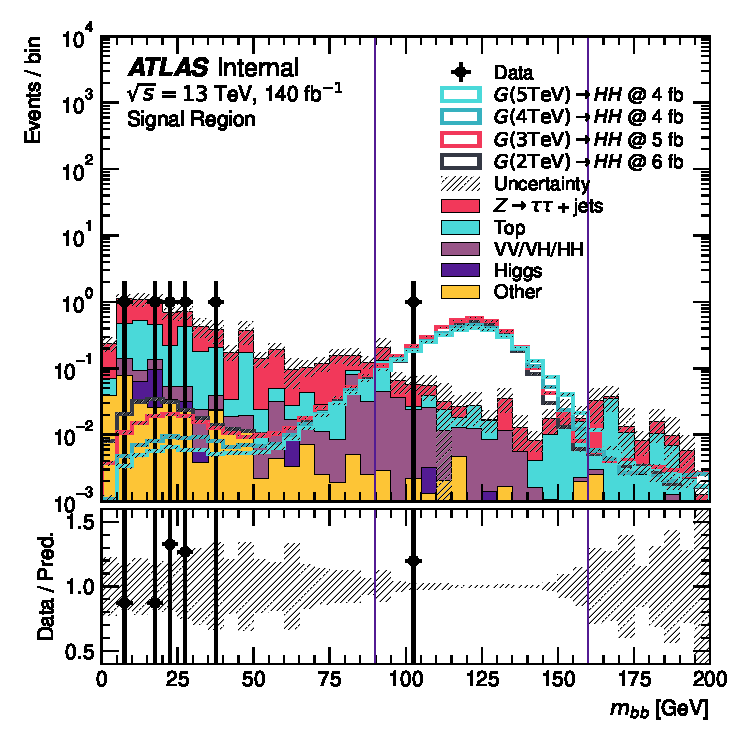
\includegraphics[width=0.50\textwidth]{kinematics_ub/M_bb_SR.pdf}
            \label{fig:SR_mbb}
        }
        %\hfill
        \subfloat[]{
            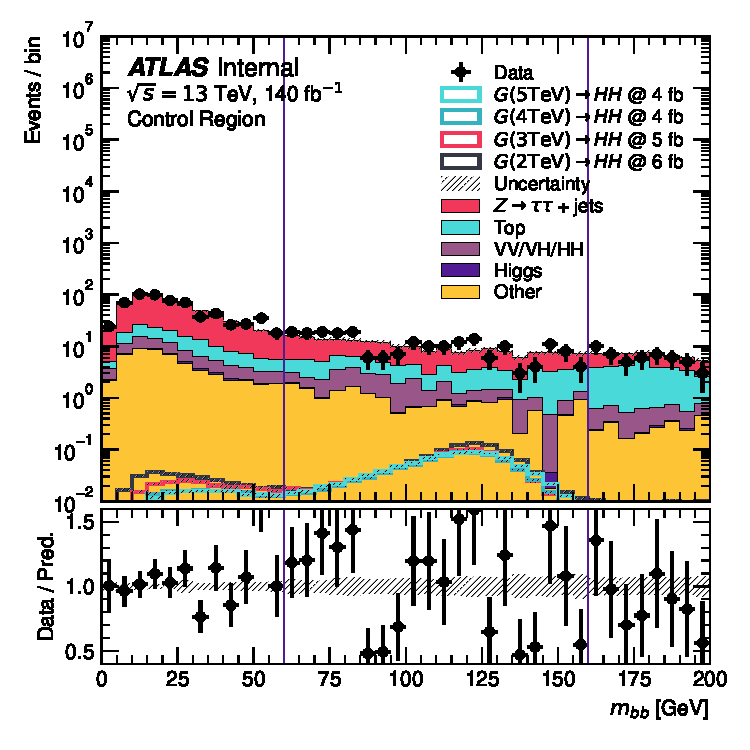
\includegraphics[width=0.50\textwidth]{kinematics_ub/M_bb_CR.pdf}
            \label{fig:CR_mbb}
        }
        \caption{
            The distribution of the $\mbb$ in the SR (\protect\subref{fig:SR_mbb}), and CR (\protect\subref{fig:CR_mbb}).
        }
        \label{fig:mbb}
    \end{figure}
    \begin{figure}[htbp]
        \centering
        \subfloat[]{
            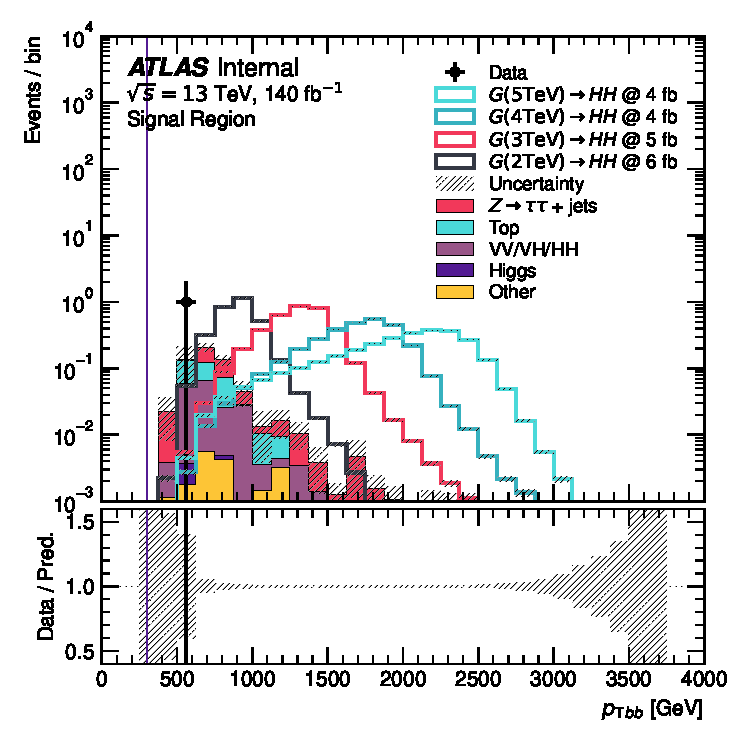
\includegraphics[width=0.50\textwidth]{kinematics_ub/pT_bb_SR.pdf}
            \label{fig:SR_pTbb}
        }
        %\hfill
        \subfloat[]{
            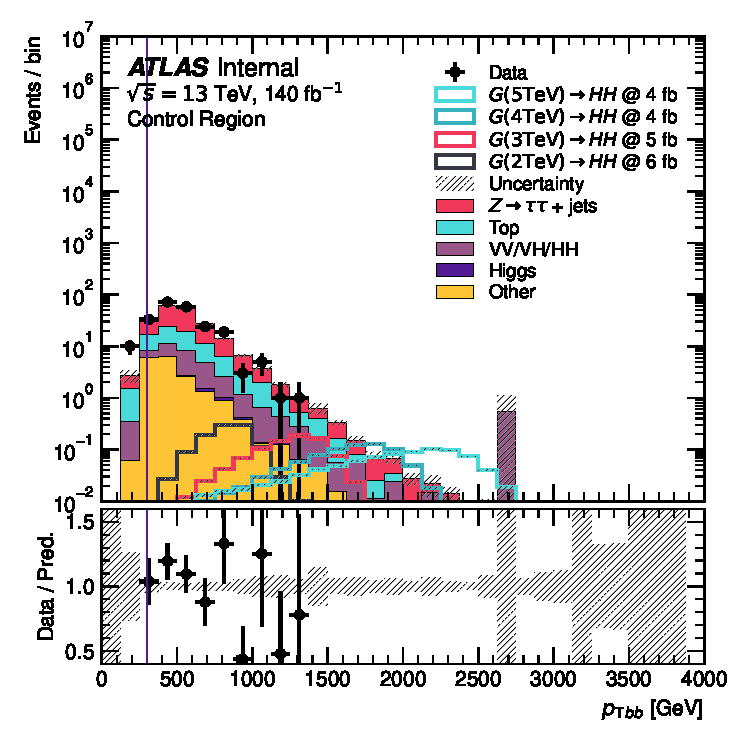
\includegraphics[width=0.50\textwidth]{kinematics_ub/pT_bb_CR.pdf}
            \label{fig:CR_pTbb}
        }
        \caption{
            The distribution of the $\ptbb$ in the SR (\protect\subref{fig:SR_pTbb}), and CR (\protect\subref{fig:CR_pTbb}).
            The $\ptbb$ distribution extends to lower values in the CR than in the SR due to the relaxed $\mttcol$ and $\mbb$ requirements.  
            This is because lower values of $\mttcol$ and $\mbb$ in the CR allow di-$\tau$ and $b\bar{b}$ systems at 
            lower $\pt$ to be produced whilst still satisfying the condition $\Delta{R} < 0.4$.
        }
        \label{fig:pTbb}
    \end{figure}
    \begin{figure}[htbp]
        
        \centering
        \subfloat[]{
            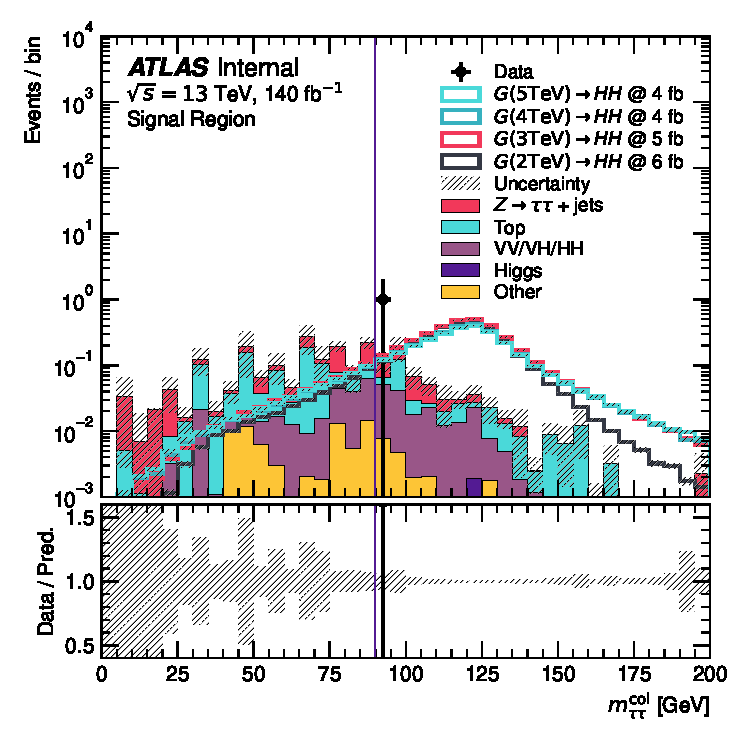
\includegraphics[width=0.50\textwidth]{kinematics_ub/M_tt_SR.pdf}
            \label{fig:SR_mtt}
        }
        %\hfill
        \subfloat[]{
            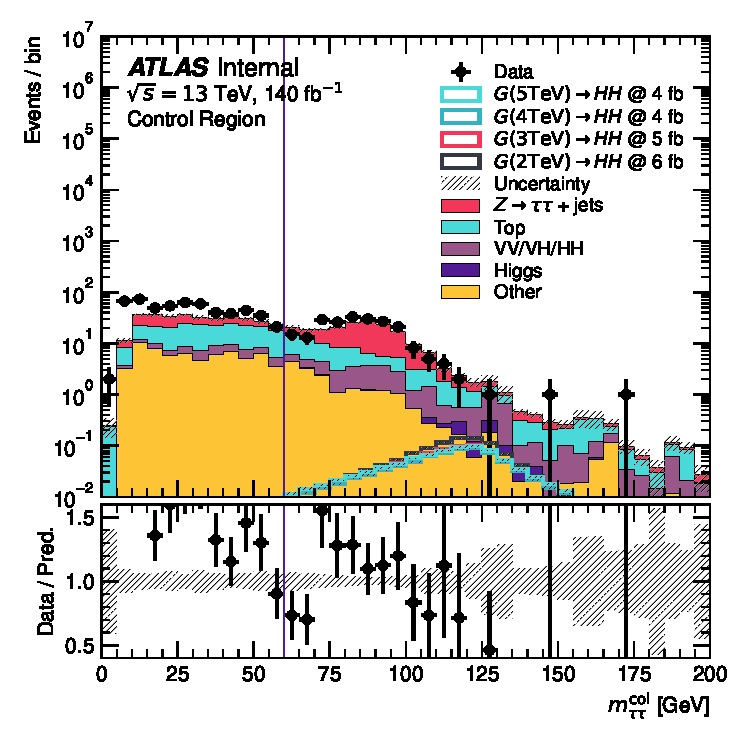
\includegraphics[width=0.50\textwidth]{kinematics_ub/M_tt_CR.pdf}
            \label{fig:CR_mtt}
        }
        \caption{
            The distribution of the $\mttcol$ in the SR (\protect\subref{fig:SR_mtt}), and CR (\protect\subref{fig:CR_mtt}).
        }
        \label{fig:mtt}
    \end{figure}   
    \begin{figure}[htbp]
        \centering
        \subfloat[]{
            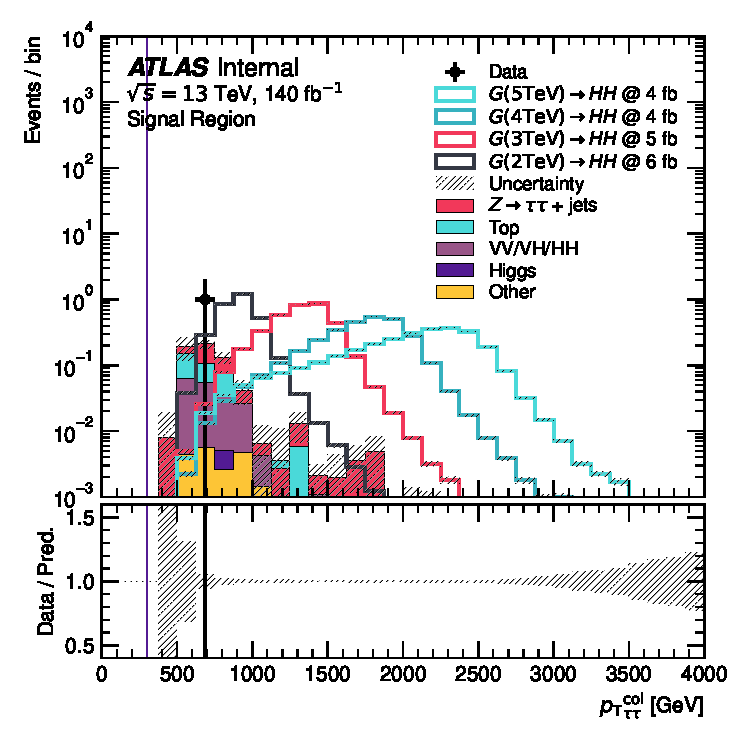
\includegraphics[width=0.50\textwidth]{kinematics_ub/pT_tt_SR.pdf}
            \label{fig:SR_pTtt}
        }
        %\hfill
        \subfloat[]{
            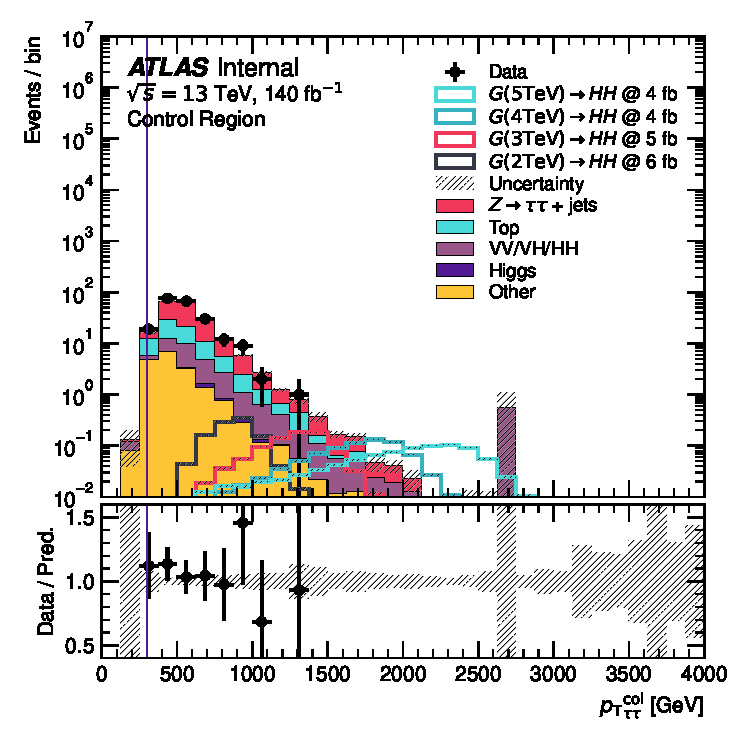
\includegraphics[width=0.50\textwidth]{kinematics_ub/pT_tt_CR.pdf}
            \label{fig:CR_pTtt}
        }
        \caption{
            The distribution of the $\pttt$ in the SR (\protect\subref{fig:SR_pTtt}), and CR (\protect\subref{fig:CR_pTtt}).
            The $\pttt$ distribution extends to lower values in the CR than in the SR due to the relaxed $\mttcol$ and $\mbb$ requirements.  
            This is because lower values of $\mttcol$ and $\mbb$ in the CR allow di-$\tau$ and $b\bar{b}$ systems at 
            lower $\pt$ to be produced whilst still satisfying the condition $\Delta{R} < 0.4$.
        }
        \label{fig:pTtt}
    \end{figure}
    \begin{figure}[htbp]
        \centering
        \subfloat[]{
            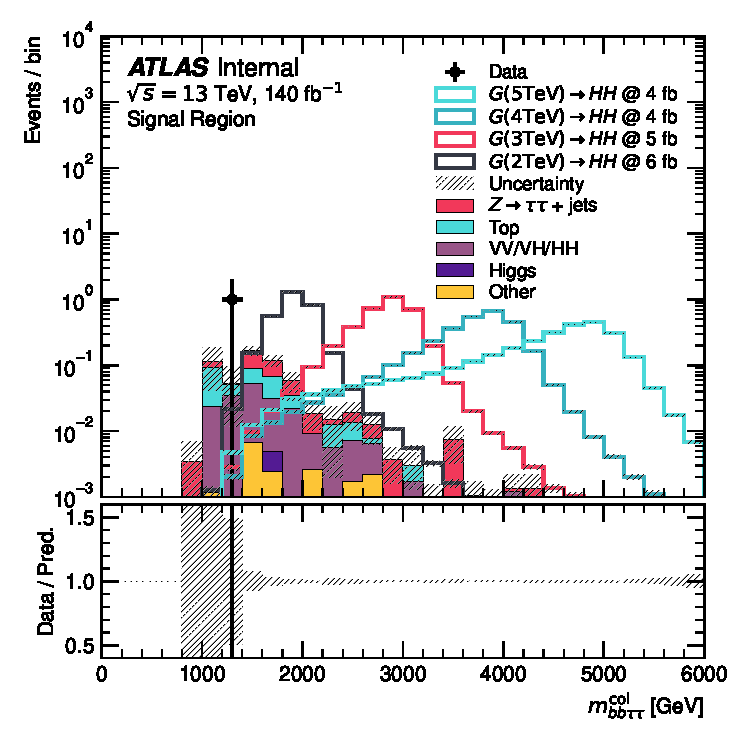
\includegraphics[width=0.50\textwidth]{kinematics_ub/M_bbtt_SR.pdf}
            \label{fig:SR_mbbtt}
        }
        %\hfill
        \subfloat[]{
            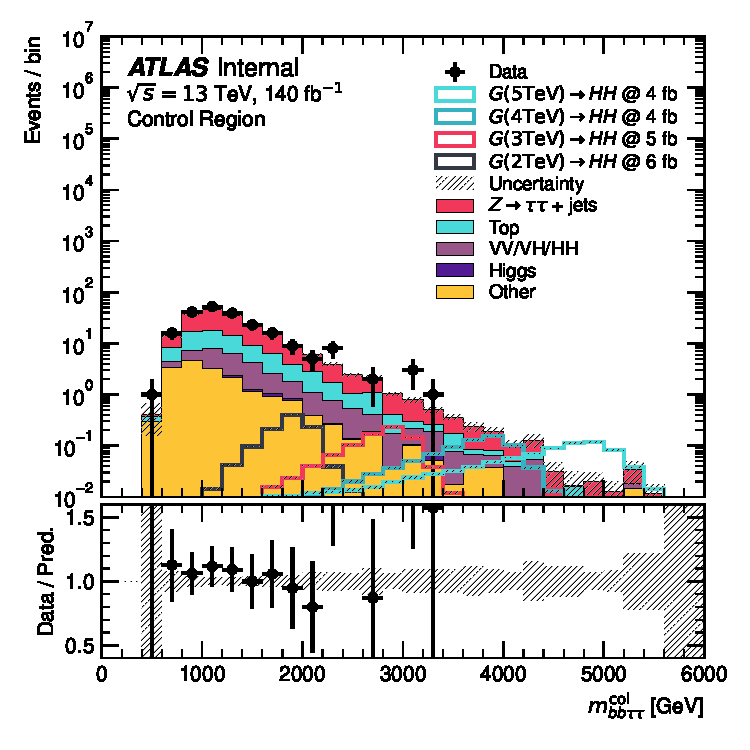
\includegraphics[width=0.50\textwidth]{kinematics_ub/M_bbtt_CR.pdf}
            \label{fig:CR_mbbtt}
        }
        \caption{
            The distribution of the $\mbbttcol$ in the SR (\protect\subref{fig:SR_mbbtt}), and CR (\protect\subref{fig:CR_mbbtt}).
            The $\mbbttcol$ distribution extends to lower values in the CR than in the SR due to the relaxed $\mttcol$ and $\mbb$ requirements.  
            This is because lower values of $\mttcol$ and $\mbb$ in the CR allow di-$\tau$ and $b\bar{b}$ systems at 
            lower $\pt$ to be produced whilst still satisfying the condition $\Delta{R} < 0.4$.
        }
        \label{fig:mbbtt}
    \end{figure}
    \begin{figure}[htbp]
        
        \centering
        \subfloat[]{
            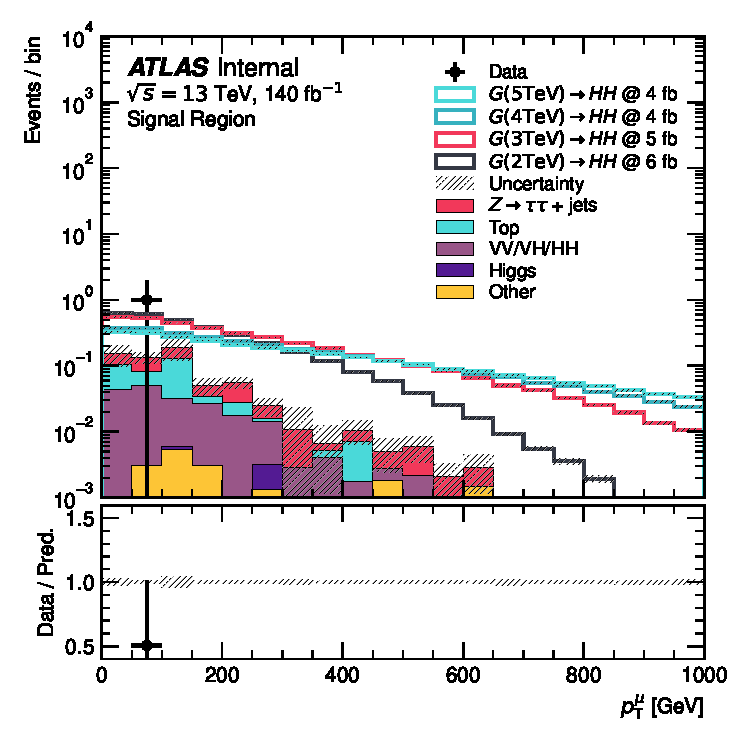
\includegraphics[width=0.50\textwidth]{kinematics_ub/pt_muon_SR.pdf}
            \label{fig:SR_pTmu}
        }
        %\hfill
        \subfloat[]{
            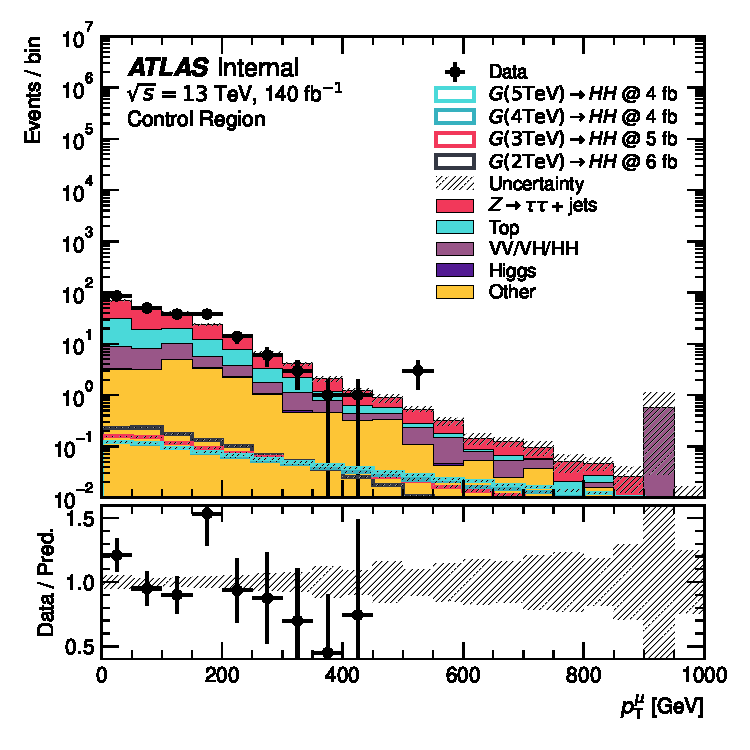
\includegraphics[width=0.50\textwidth]{kinematics_ub/pt_muon_CR.pdf}
            \label{fig:CR_pTmu}
        }
        \caption{
            The distribution of the $\ptmuon$ in the SR (\protect\subref{fig:SR_pTmu}), and CR (\protect\subref{fig:CR_pTmu}).
        }
        \label{fig:pTmu}
    \end{figure}
    \begin{figure}[htbp]
        \centering
        \subfloat[]{
            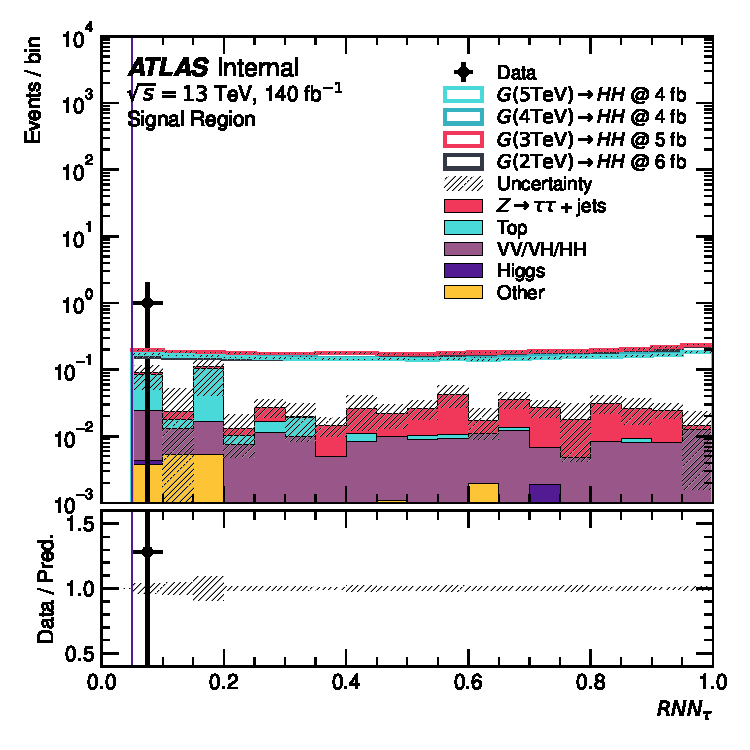
\includegraphics[width=0.50\textwidth]{kinematics_ub/tau_RNN_SR.pdf}
            \label{fig:SR_tau_rnn}
        }
        %\hfill
        \subfloat[]{
            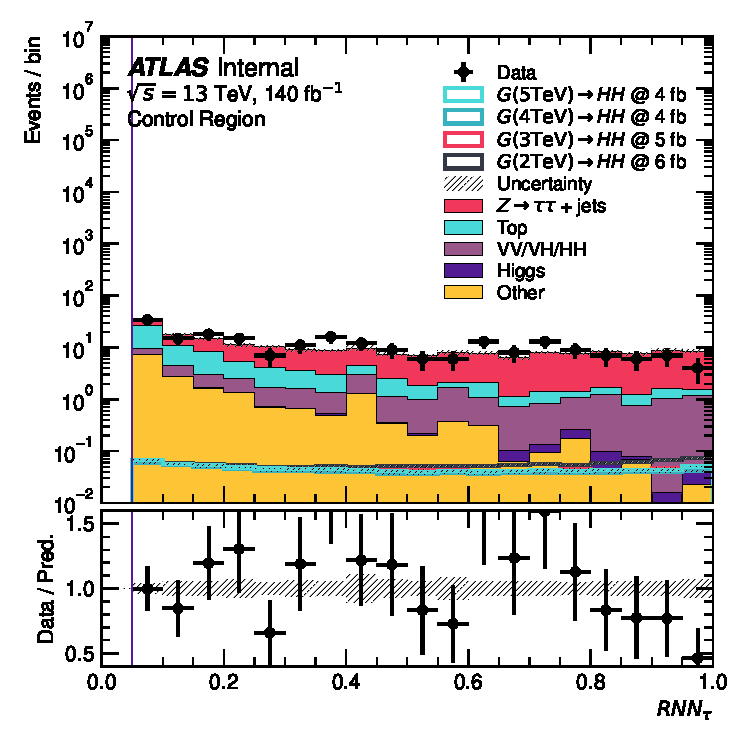
\includegraphics[width=0.50\textwidth]{kinematics_ub/tau_RNN_CR.pdf}
            \label{fig:CR_tau_rnn}
        }
        \caption{
            The distribution of the $\rnn$ in the SR (\protect\subref{fig:SR_tau_rnn}), and CR (\protect\subref{fig:CR_tau_rnn}).
        }
        \label{fig:tau_rnn}
    \end{figure}
    \begin{figure}[htbp]
        \centering
        \subfloat[]{
            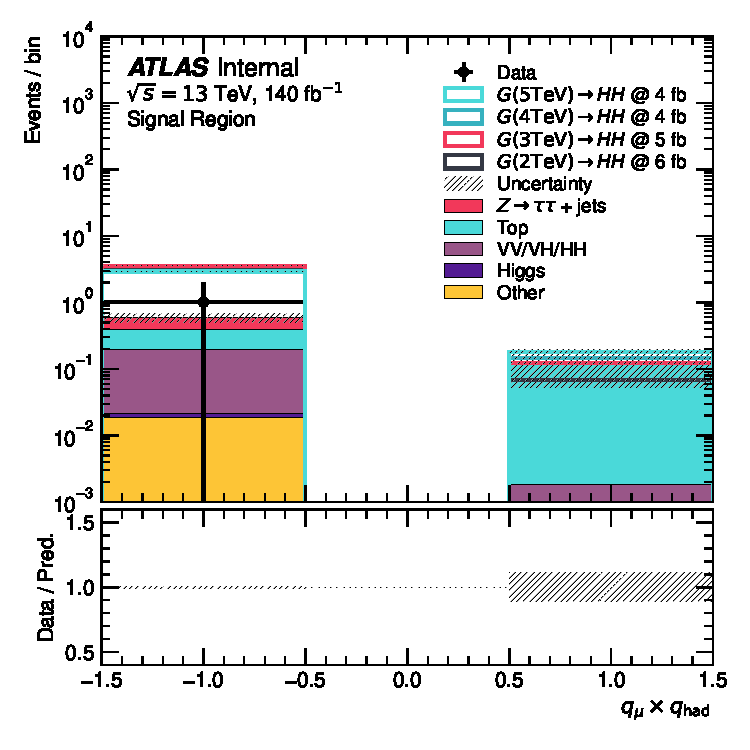
\includegraphics[width=0.50\textwidth]{kinematics_ub/qmu_qhad_SR.pdf}
            \label{fig:SR_qq}
        }
        %\hfill
        \subfloat[]{
            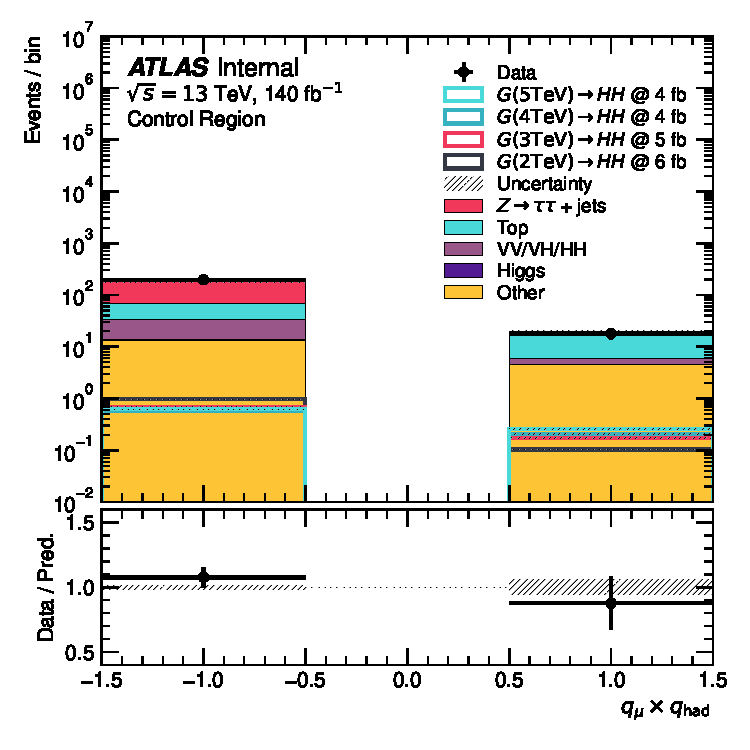
\includegraphics[width=0.50\textwidth]{kinematics_ub/qmu_qhad_CR.pdf}
            \label{fig:CR_qq}
        }
        \caption{
            The distribution of the product of the $\tau\tau$ charges in the SR (\protect\subref{fig:SR_qq}), and CR (\protect\subref{fig:CR_qq}).
        }
        \label{fig:qq}
    \end{figure}

\section{Systematic uncertainties}\label{sec:grav:sys}
    As a conservative estimation, the following systematic uncertainties are considered:
    \begin{itemize}
        \item Jet energy scale and resolution, tau energy scale and resolution, \(\MET\) and other experimental uncertainties (20\%): 
            These uncertainties can shift the reconstructed \( m_{bb\tau\tau}^{\text{col}} \) spectrum by altering the measured energies 
            and momenta of jets, \(\tau\) leptons, and the missing transverse energy. A 20\% overall uncertainty is used here as a 
            placeholder, guided by typical variations observed in similar analyses at this stage of development. 
            In a more detailed study, each of these sources would be evaluated separately through systematic variations 
            of calibration constants, comparison to data-driven control samples, and application of smearing 
            and scaling factors, then combined into a total systematic uncertainty following standard procedures.
        
        \item Theoretical uncertainties in the background cross sections, luminosity, and other parameters (50\%):
            The theoretical cross section calculations for background processes come with an intrinsic uncertainty, 
            which can be further affected by PDF variations, scale variations, and higher-order corrections. 
            We also include here uncertainties on the integrated luminosity measurement. 
            In this preliminary search, we assign a large 50\% systematic uncertainty to cover these effects conservatively. 
            As the analysis matures, these uncertainties would typically be reduced using more accurate theoretical 
            predictions and improved luminosity calibrations.
        
        \item Theoretical uncertainties in the signal modelling, GN2x identification efficiency (\( {}^{+15\%}_{-20\%} \)), 
            \(\tauhadmurm\) reconstruction and identification efficiency (12\%), and other parameters (20\%):
            For the signal process, uncertainties arise from theoretical cross section calculations and parton shower 
            modeling, which affect the predicted event rates and kinematics. Additional uncertainties stem from 
            experimental efficiencies—for instance, the GN2x \( x_{bb} \) tagger performance and the 
            \(\tauhadmurm\) reconstruction and identification efficiency. Although each of these sources 
            could in principle be evaluated separately through specialized studies (using tag-and-probe methods or dedicated control regions), 
            we have here grouped them into a single combined uncertainty. 
            We assign a conservative 20\% overall normalization uncertainty to account for possible deviations 
            in the modeling and reconstruction, while specifically quoting the GN2x identification efficiency 
            uncertainty as \( {}^{+15\%}_{-20\%} \) and the \(\tau\)-ID uncertainty as 12\%. In the future, 
            once the GN2x tagger calibration is fully validated, these uncertainties can be refined and broken down more precisely.
    \end{itemize}
    The final SM background yield in the signal region (SR) is \( 0.7 \pm 0.1 \,\text{(stat.)} \pm 0.3 \,\text{(syst.)}\). 
    Again, these systematic uncertainties are intentionally chosen to be conservative “placeholder” values. 
    Our preliminary investigations indicate that the largest systematic uncertainty will come from 
    the new GN2x \(x_{bb}\) tagger, which is still under development and not yet fully calibrated. 
    Once its performance is characterised in more detail, we expect to revisit and refine the 
    individual systematic sources---jet and tau energy scales, cross-section normalizations, tagger efficiencies, etc. 
    using the standard suite of techniques. 
    At that point, each source of uncertainty can be quantified more rigorously, substantially reducing 
    the overall uncertainty on both the background prediction and the signal acceptance.

\section{Interpretation}\label{sec:grav:interp}
    A statistical model is used to interpret the results, performing a binned likelihood fit to the data. 
    The likelihood model is constructed with the pyhf package~\cite{pyhf_joss}. 
    Given the low number of events in the signal-region, the asymptotic approximation in the likelihood model is not reliable. 
    Instead, the five-bin SR $\mbbttcol$ histogram is used as the probability density function (PDF) for the signal and background. 
    Using this PDF, we generate 10000 toy-based experiments with and without signal contributions to estimate the empirical 
    $\CLsb$ and $\CLb$~\cite{Read:2002hq} distributions, respectively. 
    From these distributions, the expected 95\% CL limits on $\sigmaGHH$ are calculated based on the 95th percentile of the empirical $\CLs$ distribution.
    The limits obtained using the asymptotic approximation are included to illustrate the disagreement between the two methods in the low-statistics regime.
    The expected 95\% CL limits on $\sigmaGHH$ at various mass points are shown in Figure~\ref{fig:limits}. 
    The expected limits are shown as the dotted black line. 
    The $\pm 1\sigma$ and $\pm 2\sigma$ bands are depicted as shaded regions around the expected limits. 
    The black solid lines show the observed limits. 
    The expected and observed upper limits, as well as the predicted cross-sections, are presented in Table~\ref{tab:limits}.

    \begin{figure}[htbp]
        \centering
        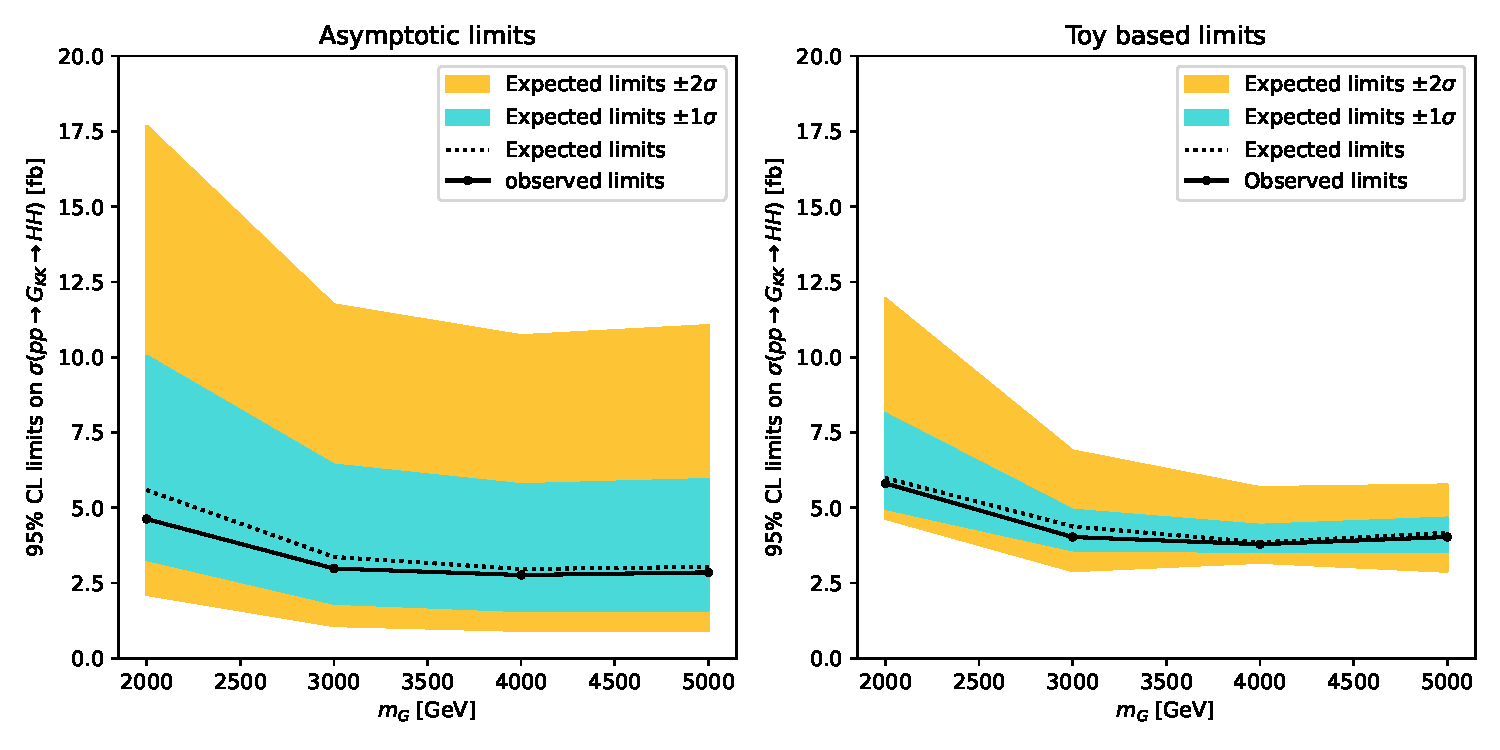
\includegraphics[width=1.0\textwidth]{limits_ub/limits_all.pdf}
        \caption{
            The expected 95\% CL limits on the $\sigmaGHH$ on various mass points. 
            The expected limits are shown as the dotted line. 
            The $\pm 1\sigma$ and $\pm 2\sigma$ bands are shown as the shaded regions around the expected limits.
            The marked solid lines show the observed limits.
        }
        \label{fig:limits}
    \end{figure}

    \begin{table}[htbp]
    \caption{The expected and observed 95\% CL limits on the $\sigma(G\rightarrow HH)$ on various mass points.}
    \label{tab:limits}
    \centering
    % \scriptsize
    \begin{tabular}{lrrrrrr}
        \toprule
        Mass [GeV] & $-2\sigma$ [fb]   & $-1\sigma$ [fb]   & Exp. [fb]   & $+1\sigma$ [fb]   & $+2\sigma$ [fb] & Observed [fb]\\
        \midrule
        2000       & 4.6               & 5.5               & 6.1         & 8.9               & 13.2            & 5.8\\
        3000       & 3.0               & 4.3               & 4.5         & 4.9               & 6.8             & 4.0\\
        4000       & 3.5               & 3.7               & 4.0         & 4.7               & 6.1             & 3.8\\
        5000       & 3.2               & 3.6               & 4.0         & 4.9               & 6.0             & 4.0\\
        \bottomrule
    \end{tabular}
\end{table}

\FloatBarrier

\section{Conclusion}\label{sec:grav:conc}
    In this analysis, we have conducted an investigation into the $G \rightarrow HH \rightarrow b\bar{b}\tau\tau$ 
    process using the full ATLAS Run-2 dataset, collected at \(\sqrt{s} = 13\)~TeV with an integrated luminosity of 140~\ifb. 
    The search benefits from advancements in the ATLAS Combined Performance, 
    particularly the GNN-based $b\bar{b}$-jet tagging algorithm and the muon-removal technique for $\tauhad$ identification. 
    The event-selection was optimised to enhance signal sensitivity while maintaining a near zero background level.

    Our results demonstrate good agreement between the data and the MC simulations in the CR, 
    indicating negligible QCD background contamination in the SR. 
    Statistical and systematic uncertainties were evaluated and incorporated into the final upper limits.

    The 95\% CL limits on $\sigmaGHH$ are derived for mass points ranging from 2 to 5~TeV. 
    Notably, the limits from this search are more than ten times better than the previous ATLAS search in the $b\bar{b}\tau\tau$ channel. 
    For instance, at a resonance mass of 3000~GeV, we obtained a limit of 3.8~fb, compared to the previous limit of approximately 55~fb 
    in the $\hhbbthth$ channel. 
    However, our limits are less stringent than those obtained in the $b\bar{b}b\bar{b}$ channel, 
    primarily due to the lower branching ratio of the $\hhbbtmth$ process. 
    With the two lepton removal reconstruction methods, boosted di-tau systems can now be reconstructed for all three channels --- $\tmth$, $\teth$ and $\thth$.
    These algorithm advancements could position ATLAS to approach the 1~fb limits set by the $\hhbbbb$ channel with all three sub-channels, 
    especially considering the significantly lower background in the $\hhbbtt$ final state.
